% ------------------------------------------------------------------------
% ------------------------------------------------------------------------
% Modelo UFSC para Trabalhos Academicos (tese de doutorado, dissertação de
% mestrado) utilizando a classe abntex2
%
% Autor: Alisson Lopes Furlani
% 	Modificações:
%	- 27/08/2019: Alisson L. Furlani, add pacote 'glossaries' para listas
%   - 06/11/2019: Luiz-Rafael Santos, modifica para Trabalho de Conclusão de Curso
% ------------------------------------------------------------------------
% ------------------------------------------------------------------------

\documentclass[
	% -- opções da classe memoir --
	12pt,				% tamanho da fonte
	%openright,			% capítulos começam em pág ímpar (insere página vazia caso preciso)
	oneside,			% para impressão no anverso. Oposto a twoside
	a4paper,			% tamanho do papel. 
	% -- opções da classe abntex2 --
	chapter=TITLE,		% títulos de capítulos convertidos em letras maiúsculas
	section=TITLE,		% títulos de seções convertidos em letras maiúsculas
	%subsection=TITLE,	% títulos de subseções convertidos em letras maiúsculas
	%subsubsection=TITLE,% títulos de subsubseções convertidos em letras maiúsculas
	% -- opções do pacote babel --
	english,			% idioma adicional para hifenização
	%french,				% idioma adicional para hifenização
	%spanish,			% idioma adicional para hifenização
	brazil				% o último idioma é o principal do documento
	]{abntex2}

\usepackage{setup/ufscthesisA4-alf}

\usepackage[alf]{abntex2cite}

% ---
% Filtering and Mapping Bibliographies
% ---
% Pacotes de citações
% ---
\usepackage{csquotes}
\usepackage[backend = biber, style = abnt]{biblatex}
% FIXME Se desejar estilo numérico de citações,  comente a linha acima e descomente a linha a seguir.
% \usepackage[backend = biber, style = numeric-comp]{biblatex}

% Packages for pseudocode algorithms
\usepackage[portuguese,linesnumbered,lined]{algorithm2e}

\usepackage{mathtools}

\setlength\bibitemsep{\baselineskip}
\DeclareFieldFormat{url}{Disponível~em:\addspace\url{#1}}
\NewBibliographyString{sineloco}
\NewBibliographyString{sinenomine}
\DefineBibliographyStrings{brazil}{%
	sineloco     = {\mkbibemph{S\adddot l\adddot}},
	sinenomine   = {\mkbibemph{s\adddot n\adddot}},
	andothers    = {\mkbibemph{et\addabbrvspace al\adddot}},
	in			 = {\mkbibemph{In:}}
}

\addbibresource{aftertext/references.bib} % Seus arquivos de referências

% ---
\DeclareSourcemap{
	\maps[datatype=bibtex]{
		% remove fields that are always useless
		\map{
			\step[fieldset=abstract, null]
			\step[fieldset=pagetotal, null]
		}
		% remove URLs for types that are primarily printed
%		\map{
%			\pernottype{software}
%			\pernottype{online}
%			\pernottype{report}
%			\pernottype{techreport}
%			\pernottype{standard}
%			\pernottype{manual}
%			\pernottype{misc}
%			\step[fieldset=url, null]
%			\step[fieldset=urldate, null]
%		}
		\map{
			\pertype{inproceedings}
			% remove mostly redundant conference information
			\step[fieldset=venue, null]
			\step[fieldset=eventdate, null]
			\step[fieldset=eventtitle, null]
			% do not show ISBN for proceedings
			\step[fieldset=isbn, null]
			% Citavi bug
			\step[fieldset=volume, null]
		}
	}
}
% ---

% ---
% Informações de dados para CAPA e FOLHA DE ROSTO
% ---
\autor{João Vitor Maia Neves Cordeiro}
\titulo{Desenvolvimento de uma técnica de esteganografia explorando arquivos binários de código compilado.}

% Caso não tenha substítulo, comente a linha a seguir.
%\subtitulo{Subtítulo (se houver)}

% FIXME Substituir 'XXXXXX' pelo nome do seu
% orientador.
\orientador{Prof. Jean Everson Martina, Dr.}
% \orientador[Orientadora]{Nome da orientadora, Dra.}
% coorientador. Caso não tenha coorientador, comente a linha a seguir.
%\coorientador{Prof. XXXXXX, Dr.}
% \coorientador[Coorientadora]{XXXXXX, Dra.}
% programa/curso.
\coordenador{Prof. Jean Everson Martina, Dr.}
% FIXME Se for coordenadora mulher, comente a linha acima e descomente a linha a seguir.
% \coordenador[Coordenadora]{Nome da Coordenadora, Dra.}
% FIXME Substituir '[ano da entrega]' pelo ano (ano) em que seu trabalho foi defendido.
\ano{2023}
% FIXME Substituir '[dia] de [mês] de [ano]' pela data em que ocorreu sua defesa.
\data{[dia] de [mês] de [ano]}
% FIXME Substituir '[Cidade da defesa]' pela cidade em que ocorreu sua defesa.
\local{Florianópolis}
\instituicaosigla{UFSC}
\instituicao{Universidade Federal de Santa Catarina}
% FIXME Substituir 'Dissertação/Tese' pelo tipo de trabalho (Tese, Dissertação). 
\tipotrabalho{Trabalho de Conclusão de Curso}
% FIXME Substituir '[licenciado/bacharel] em [nome do título obtido]' pela grau adequado.
\formacao{bacharel em Ciência da Computação}
% FIXME Substituir '[licenciado/bacharel]' pelo nivel adequado.
\nivel{bacharel}
% FIXME Substituir 'Curso de Graduação em [XXXXXXXX]' pela curso adequado.
\programa{Curso de Graduação em Ciência da Computação}
% FIXME Substituir 'Campus XXXXXX ou Centro de XXXXXX' pelo campus ou centro adequado.
\centro{Campus Florianópolis}
\preambulo
{%
\imprimirtipotrabalho~do~\imprimirprograma~do~\imprimircentro~da~\imprimirinstituicao~para~a~obtenção~do~título~de~\imprimirformacao.
}
% ---

% ---
% Configurações de aparência do PDF final
% ---
% alterando o aspecto da cor azul
\definecolor{blue}{RGB}{41,5,195}
% informações do PDF
\makeatletter
\hypersetup{
     	%pagebackref=true,
		pdftitle={\@title}, 
		pdfauthor={\@author},
    	pdfsubject={\imprimirpreambulo},
	    pdfcreator={LaTeX with abnTeX2},
		pdfkeywords={ufsc, latex, abntex2}, 
		colorlinks=true,       		% false: boxed links; true: colored links
    	linkcolor=black,%blue,          	% color of internal links
    	citecolor=black,%blue,        		% color of links to bibliography
    	filecolor=black,%magenta,      		% color of file links
		urlcolor=black,%blue,
		bookmarksdepth=4
}
\makeatother
% ---

% ---
% compila a lista de abreviaturas e siglas e a lista de símbolos
% ---

% Declaração das siglas
\siglalista{ELF}{Executable and Linkable File}
\siglalista{PE}{Portable Executable}
\siglalista{ISA}{Instruction Set Architecture}
\siglalista{CISC}{Complex Instruction Set Computer}
\siglalista{RISC}{Reduced Instruction Set Computer}
\siglalista{ARM}{Advanced RISC Machine}
\siglalista{ROP}{Return Oriented Programming}

% Declaração dos simbolos
\simbololista{C}{\ensuremath{C}}{Circunferência de um círculo}
\simbololista{pi}{\ensuremath{\pi}}{Número pi} 
\simbololista{r}{\ensuremath{r}}{Raio de um círculo}
\simbololista{A}{\ensuremath{A}}{Área de um círculo}

\usepackage{listings}
\usepackage{xcolor}

\definecolor{codegreen}{rgb}{0,0.6,0}
\definecolor{codegray}{rgb}{0.5,0.5,0.5}
\definecolor{codepurple}{rgb}{0.58,0,0.82}
\definecolor{backcolour}{rgb}{1,1,1}

\lstdefinestyle{code_style}{
    backgroundcolor=\color{backcolour},   
    commentstyle=\color{codegreen},
    keywordstyle=\color{magenta},
    numberstyle=\tiny\color{codegray},
    stringstyle=\color{codepurple},
    basicstyle=\ttfamily\footnotesize,
    breakatwhitespace=false,         
    breaklines=true,                 
    captionpos=b,                    
    keepspaces=true,                 
    numbers=left,                    
    numbersep=5pt,                  
    showspaces=false,                
    showstringspaces=false,
    showtabs=false,                  
    tabsize=2
}

\lstset{style=code_style}


% compila a lista de abreviaturas e siglas e a lista de símbolos
\makenoidxglossaries 

% ---

% ---
% compila o indice
% ---
\makeindex
% ---

% ----
% Início do documento
% ----
\begin{document}

% Seleciona o idioma do documento (conforme pacotes do babel)
%\selectlanguage{english}
\selectlanguage{brazil}

% Retira espaço extra obsoleto entre as frases.
\frenchspacing 

% Espaçamento 1.5 entre linhas
\OnehalfSpacing

% Corrige justificação
%\sloppy

% ----------------------------------------------------------
% ELEMENTOS PRÉ-TEXTUAIS
% ----------------------------------------------------------
% \pretextual %a macro \pretextual é acionado automaticamente no início de \begin{document}
% ---
% Capa, folha de rosto, ficha bibliografica, errata, folha de apróvação
% Dedicatória, agradecimentos, epígrafe, resumos, listas
% ---
% ---
% Capa
% ---
\imprimircapa
% ---

% ---
% Folha de rosto
% (o * indica que haverá a ficha bibliográfica)
% ---
\imprimirfolhaderosto*
% ---

% ---
% Inserir a ficha bibliografica
% ---
% http://ficha.bu.ufsc.br/
\begin{fichacatalografica}
	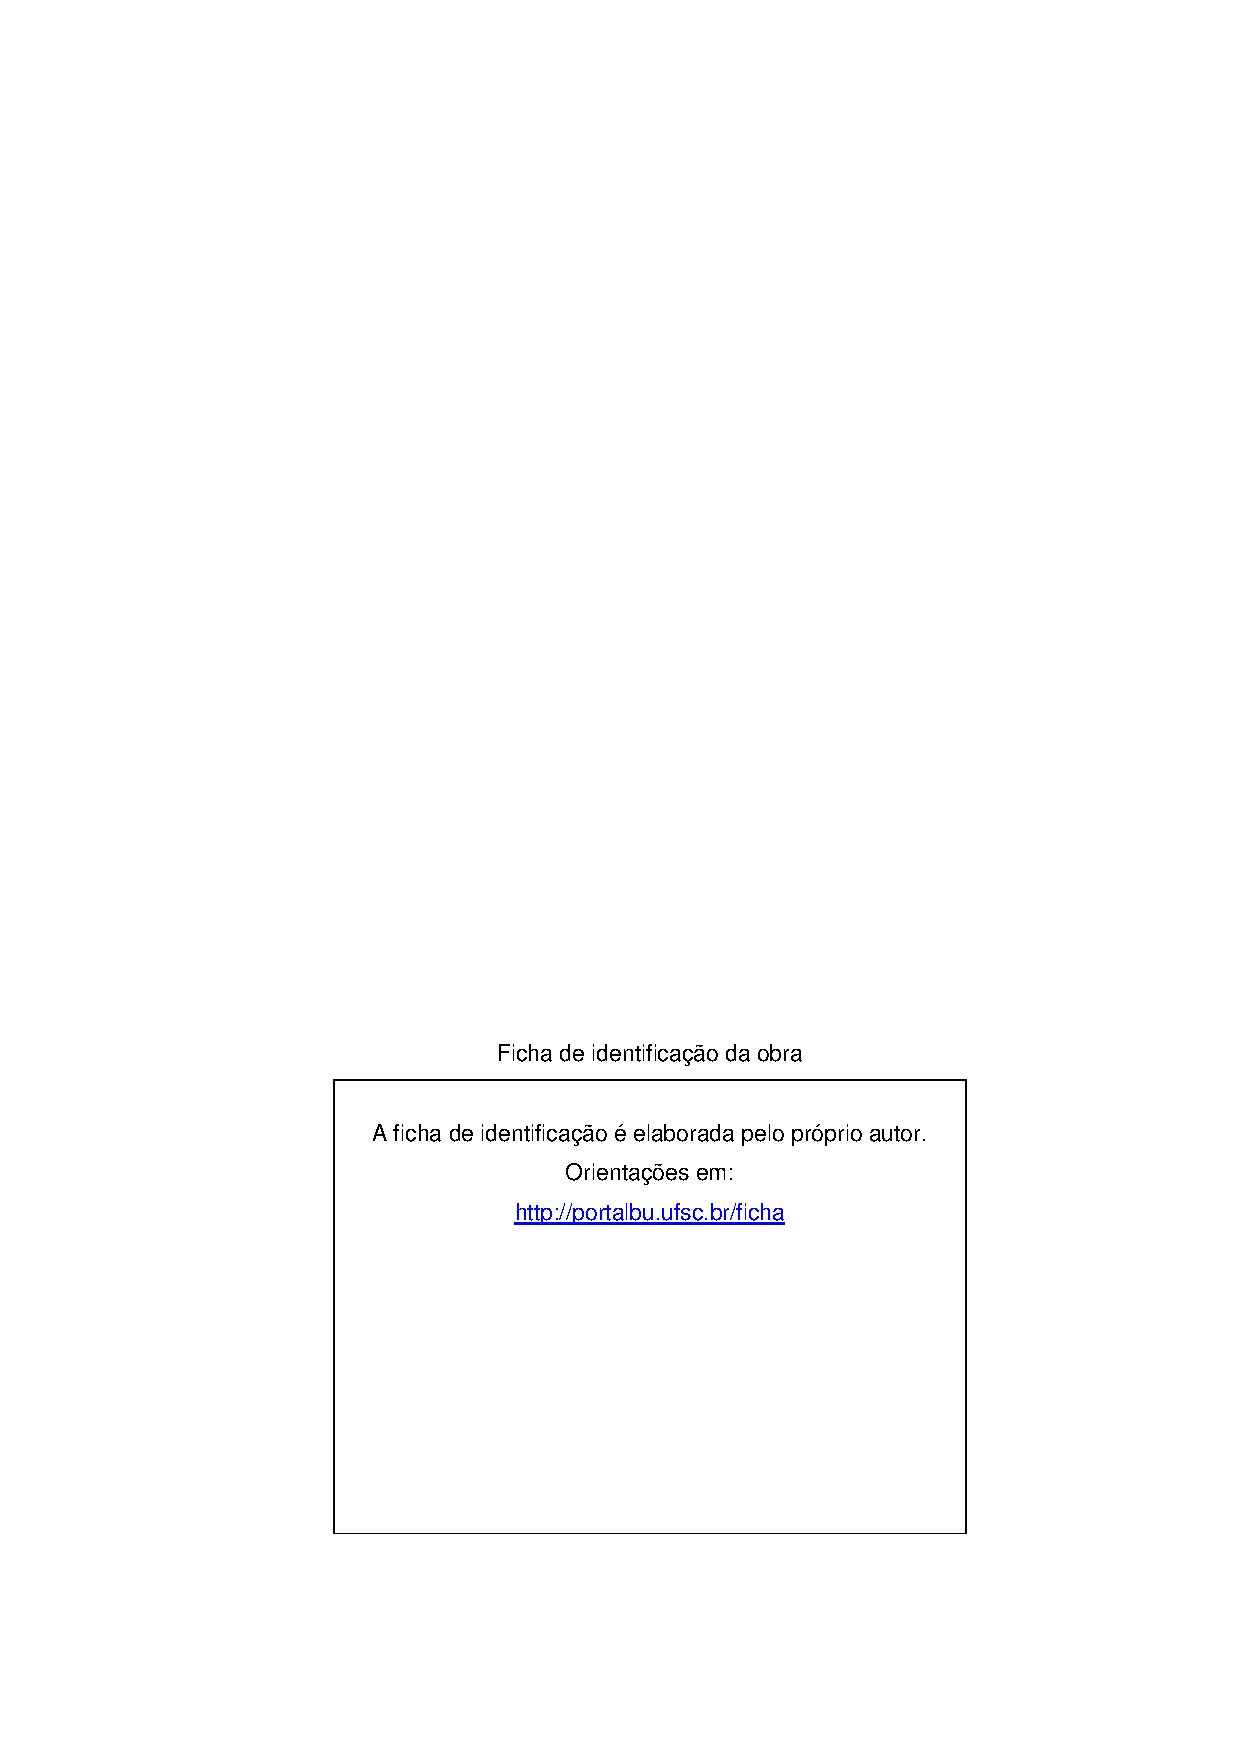
\includepdf{beforetext/Ficha_Catalografica.pdf}
\end{fichacatalografica}
% ---

% ---
% Inserir folha de aprovação
% ---
\begin{folhadeaprovacao}
	\OnehalfSpacing
	\centering
	\imprimirautor\\%
	\vspace*{10pt}		
	\textbf{\imprimirtitulo}%
	\ifnotempty{\imprimirsubtitulo}{:~\imprimirsubtitulo}\\%
	%		\vspace*{31.5pt}%3\baselineskip
	\vspace*{\baselineskip}
	%\begin{minipage}{\textwidth}
	% ~do~\imprimirprograma~do~\imprimircentro~da~\imprimirinstituicao~para~a~obtenção~do~título~de~\imprimirformacao.
	Este~\imprimirtipotrabalho~foi julgado adequado para obtenção do Título de “\imprimirformacao” e aprovado em sua forma final pelo~\imprimirprograma. \\
		\vspace*{\baselineskip}
	\imprimirlocal, \imprimirdata. \\
	\vspace*{2\baselineskip}
	\assinatura{\OnehalfSpacing\imprimircoordenador \\ \imprimircoordenadorRotulo~do Curso}
	\vspace*{2\baselineskip}
	\textbf{Banca Examinadora:} \\
	\vspace*{\baselineskip}
	\assinatura{\OnehalfSpacing\imprimirorientador \\ \imprimirorientadorRotulo}
	%\end{minipage}%
	\vspace*{\baselineskip}
	\assinatura{Prof.(a) xxxx, Dr(a).\\
	Avaliador(a) \\
	Instituição xxxx}

	\vspace*{\baselineskip}
	\assinatura{Prof.(a) xxxx, Dr(a).\\
	Avaliador(a) \\
	Instituição xxxx}


\end{folhadeaprovacao}
% ---

% ---
% Dedicatória
% ---
\begin{dedicatoria}
	\vspace*{\fill}
	\noindent
	\begin{adjustwidth*}{}{5.5cm}     
		Este trabalho é dedicado a todos que não chegaram aqui comigo.
	\end{adjustwidth*}
\end{dedicatoria}
% ---

% ---
% Agradecimentos
% ---
\begin{agradecimentos}
	Deixo meus profundos agradecimentos à minha revisora preferida, Maria Eduarda da Luz, por não deixar meus inúmeros erros passarem para o texto final; ao meu orientador Jean Everson Martina que acreditou e confiou na minha proposta inicial; ao meu professor e amigo Rodrigo Ramos Nogueira pelas companhias nas madrugadas de trabalho; e por fim a todos os meus amigos que me ajudaram a construir quem sou hoje. 
\end{agradecimentos}
% ---

% ---
% Epígrafe
% ---
\begin{epigrafe}
	\vspace*{\fill}
	\begin{flushright}
		\textit{``Apparently neutral s protest is thoroughly discounted and ignored. Isman hard hit. Blockade issue affects pretext for embargo on by-products, ejecting suets and vegetable oils.''\\
			(Espião Desconhecido, 19??)}
	\end{flushright}
\end{epigrafe}
% ---

% ---
% RESUMOS
% ---

% resumo em português
\setlength{\absparsep}{18pt} % ajusta o espaçamento dos parágrafos do resumo
\begin{resumo}
	\SingleSpacing
	A esteganografia trabalha embutindo informação dentro de outra e escondendo essa transformação ao olhar de um observador ingênuo, de forma que não seja possível distinguir a mídia original do resultado transformado. Apesar do campo já possuir técnicas consolidadas para lidar com imagens, áudios e outros tipos de mídia, quando trata-se de arquivos de código binário a literatura e o ferramental atual são escassos. Dado esse contexto, esse trabalho propõe o desenvolvimento de uma técnica robusta capaz de inserir informações dentro de um arquivo executável sem alterar a semântica do programa fonte, podendo ser utilizado para aplicações como assinatura digital de software, proteção de direitos autorais e comunicação oculta.
	
	\textbf{Palavras-chave}: estegranografia. segurança da informação.
\end{resumo}

% resumo em inglês
\begin{resumo}[Abstract]
	\SingleSpacing
	\begin{otherlanguage*}{english}
        Stegranography is the craft of embedding information inside another source of data, hiding it from an external observer. Despite the extensive research on techniques built for image, audio and text steganography, when it comes to using executable files as cover objects the academic productions and tools are scarce. This article aims to develop a new method capable of embedding information inside an executable file without altering the semantics of the source code, allowing application of the technique to generic pieces of software.
		
		\textbf{Keywords}: steganography. information security.
	\end{otherlanguage*}
\end{resumo}

{%hidelinks
	\hypersetup{hidelinks}
	% ---
	% inserir lista de ilustrações
	% ---
	\pdfbookmark[0]{\listfigurename}{lof}
	\listoffigures*
	\cleardoublepage
	% ---
	
	% ---
	% inserir lista de quadros
	% ---
	%\pdfbookmark[0]{\listofquadrosname}{loq}
	%\listofquadros*
	%\cleardoublepage
	% ---
	
	% ---
	% inserir lista de tabelas
	% ---
	%\pdfbookmark[0]{\listtablename}{lot}
	%\listoftables*
	%\cleardoublepage
	% ---
	
	% ---
	% inserir lista de abreviaturas e siglas (devem ser declarados no preambulo)
	% ---
	\imprimirlistadesiglas
	% ---
	
	% ---
	% inserir lista de símbolos (devem ser declarados no preambulo)
	% ---
	%\imprimirlistadesimbolos
	% ---
	
	% ---
	% inserir o sumario
	% ---
	\pdfbookmark[0]{\contentsname}{toc}
	\tableofcontents*
	\cleardoublepage
	
}%hidelinks
% ---
% ---

% ----------------------------------------------------------
% ELEMENTOS TEXTUAIS
% ----------------------------------------------------------
\textual

% ---
% 1 - Introdução
% ---
% ----------------------------------------------------------
\chapter{Introdução}
% ----------------------------------------------------------

Esteganografia é a nomenclatura utilizada para um conjunto de técnicas, inicialmente desenvolvidas para espionagem, que atuam escondendo uma informação dentro de uma outra mídia, de modo que a mídia criada após a manipulação seja visualmente indistinguível da original para um observador externo.

A crescente disseminação de computadores a partir do século 20 recuperou diversas técnicas analógicas de espionagem que predatam a área da computação, adicionando o poder de processamento digital para aprimorar a efetividade e as aplicações de tais técnicas. Notoriamente temos a criptografia como a principal expoente dessa transformação, estando presente na maior parte das aplicações modernas. Apesar de ser o maior caso a criptografia não foi a única área a passar por isso, as técnicas de esteganografia também foram afetadas pela introdução do fator digital \cite{JohnsonJajodia}.

Representações digitais de mídias diversas permitem que a informação seja processada e escondida de formas que uma mídia física por sua natureza não conseguiria suportar, fornecendo uma gama maior de técnicas e aplicações esteganográficas, além de permitir a combinação das técnicas mais modernas de criptografia para esconder uma mensagem cifrada.

As novas técnicas esteganográficas desenvolvidas no meio digital circulam por diversas áreas da computação, nos últimos anos destaca-se o uso no ramo de marcas d'água digitais, onde são inseridas no arquivo informações para ajudar na verificação de sua integridade, autenticidade e dados autorais. Nessas aplicações, os dados embutidos não são necessariamente secretos portanto a invisibilidade nesses casos é apenas uma propriedade opcional do algoritmo e outros fatores surgem como prioridade. Uma dessas novas características que ganham destaque é a capacidade de resistir a ataques de distorção do arquivo, mantendo os dados embutidos seguros de um atacante que queira danificar a integridade do arquivo fonte \cite{9187785}.

\section{Motivação}

Apesar de o comum ser utilizar tais técnicas em imagens, áudios e outros formatos de mídia de uso geral, os mesmos conceitos podem ser aplicados para qualquer formato de arquivo que contenha informação, ajustando ou criando novos algoritmos. Uma aplicação menos explorada atualmente é a esteganografia em arquivos de código binário, que pode ser utilizada para transmissão de mensagens secretas, marcas d'água digitais em software, verificação de integridade e autoria a partir de uma assinatura e até mesmo inclusão de trechos de código alternativo, maliciosos ou não, dentro do programa principal \cite{Weaver}.

Os softwares que consumimos diariamente muitas vezes são compilados em arquivos binários que codificam as linhas de código fonte em instruções binárias compreendidas pelo processador alvo. Esses arquivos compilados também possuem extensões e formatos, sendo os principais formatos utilizados o \emph{Executable Linkable File} (ELF) e \textit{Portable Executable} (PE), sendo que o último possuí diversas versões.

Trabalhos passados já obtiveram resultados no desenvolvimento e validação de técnicas esteganográficas em arquivos binários, notóriamente o projeto Hydan \cite{Hydan} foi um dos precursores ao criar uma técnica para a arquitetura \emph{x86} capaz de incorporar bits de informação em um arquivo na proporção de $\frac{1}{110}$. Em comparação, técnicas que se utilizam de mídias mais suscetíveis como imagens JPEG podem atingir uma eficiência de $\frac{1}{17}$, o que contribui para a aplicação de técnicas de obfuscação dentro do espaço de busca.

Em seguida novas pesquisas foram realizadas em torno da ideia inicial do Hydan, buscando aumentar a taxa de incorporação das técnicas empregadas utilizando-se de heurísticas mais efetivas \cite{ICISC04}, expondo vulnerabilidades contra ataques baseados no espaço de busca pequeno que o algoritmo gera \cite{Wright2020DetectingHS}. Entretanto, as pesquisas da área estão limitadas em dois sentidos: a falta de novas propostas de algoritmos que ampliem a capacidade de codificação por arquivo e a preocupação de tornar as técnicas já existentes disponíveis ao longo de mais plataformas, visto que os trabalhos já desenvolvidos costumam focar exclusivamente na arquitetura x86.

\section{Objetivos}

\subsection{Objetivo Geral}

Tendo em vista a atual escassez de algoritmos específicos para a utilização de arquivos binários de código fonte como estego-objetos em arquiteturas alternativas à x86, esse trabalho se propõe a desenvolver um algoritmo que atenda aos requisitos necessários para esse objetivo, demonstrando que é possível aplicar os mesmos conceitos em outras plataformas.

\subsection{Objetivos Específicos}

\begin{itemize}
    \item Pesquisar o estado da arte dos algoritmos de esteganografia utilizando arquivos de código compilado como mídia.
    \item Pesquisar e documentar brechas na arquitetura alvo que permitam a codificação de mensagens dentro de um arquivo compilado.
    \item Desenvolver um algoritmo que explore as brechas encontradas para aplicar técnicas esteganográficas em código da arquitetura alvo.
    \item Desenvolver uma aplicação que implemente o algoritmo desenvolvido.
    \item Disponibilizar a aplicação de forma pública para uso da comunidade e evolução do campo.
\end{itemize}

\section{Estrutura do Trabalho}

Além do presente capítulo introdutório, este trabalho conta com mais três capítulos, explicados a seguir.

No capítulo 2 são apresentados conceitos gerais para a compreensão da temática do trabalho e seus materiais relacionados. São superficialmente explicados noções e definições basilares sobre esteganografia e obsfucação, contendo um breve histórico da formação e avanço das ideias trabalhadas. Também neste capítulo é apresentada uma introdução sobre arquivos executáveis de código e a arquitetura RISC-V escolhida como alvo do estudo. Ao final é exposta a revisão bibliográfica utilizada como fundamentação para o trabalho.

No capítulo 3 está detalhado o desenvolvimento do trabalho, dividido em duas principais partes. A primeira parte discorre sobre a elaboração teórica do algoritmo proposto, detalhando as escolhas de projeto e aplicando uma análise de complexidade, robustez e eficiência de codificação de informação do método. Já a segunda parte detalha a implementação do algoritmo juntamente com uma aplicação com interface textual para a utilização do algoritmo.

No capítulo 4 são discutidos os resultados da implementação realizada, assim como possibilidades de trabalhos futuros a serem desenvolvidos orbitando o algoritmo desenvolvido.
% ---

% ---
% 2 - Conceituação e Revisão Bibliográfica
% ---
% ----------------------------------------------------------
\chapter{Conceituação e Revisão Bibliográfica}\label{cap:conceitos}

Ao longo deste capítulo serão introduzidos conceitos necessários para a compreensão do algoritmo proposto como objetivo, com uma pesquisa calcada tanto em materiais e documentos históricos quanto produções acadêmicas recentes de maior relevância.

\section{Conceitos Gerais}
% ----------------------------------------------------------
Nessa seção estão descritos os conceitos que a proposta desse trabalho utiliza como alicerce para a construção do objetivo definido.

\subsection{Estegranografia}

\subsubsection{Definição e Histórico}

Etimologicamente a palavra esteganografia deriva do grego, \textit{steganographia}, que significa de forma literal "escrita escondida". Historicamente a palavra já foi utilizada para definir um conjunto bem abrangente de técnicas ao decorrer dos sećulos, iniciando-se com ocultação de símbolos em placas de hieróglifos egípicios, passando por técnicas de alteração química em tintas que só seriam exibidas em determinadas circustâncias durante a Segunda Guerra Mundial e chegando nos dias atuais com o uso de algoritmos computacionais para ocultação de mensagens em arquivos digitais.

Conceitualmente, a primeira definição registrada vem do polímata Johannes Trithemius na obra \textit{Steganographia}, escrita em 1499 e publicada apenas após sua morte em 1606 em três partes. No subtítulo do tratado, originalmente em latim e traduzido por Judge, o autor alemão introduz esteganografia como a arte pela qual a escrita é escondida e requer recuperação pela mente humana \cite{judge}.

A publicação em si é uma demonstração do uso da escrita escondida, pois inicialmente foi reconhecida como um tratado sobre demonologia de teor teológico, e só após um estudo mais aprofundado foram encontradas mensagens escondidas com metodologia sofisticadas nos dois primeiros livros. O terceiro livro só foi decifrado em 1998 por Thomas Ernst \cite{ernst} e Jim Reeds \cite{reeds} que trabalharam sem conhecimento da pesquisa um do outro.

Com a evolução da área e do campo científico como um todo, se fez necessário definir esteganografia de forma menos esotérica do que a usada por Trithemius. De forma objetiva, esteganografia é o uso de qualquer processo capaz de ocultar a existência de uma mensagem em um objeto externo, tornando essa mensagem opaca para qualquer observador que não tenha o conhecimento prévio da aplicação da técnica \cite{judge}. 

Segundo Katzenbeisser (1999) podemos generalizar grande parte dos métodos esteganográficos em um princípio comum: o remetente deseja compartilhar uma mensagem secreta (\textit{m}) com um receptor pré informado, para isso ele escolhe um \textbf{objeto de cobertura} (\textit{c}) que possa ser visto como uma mensagem pública. Então, utilizando-se de algum método específico, o remetente insere \textit{m} dentro de \textit{c}. Pode-se ainda utilizar uma \textbf{estego-chave} (\textit{k}) para controlar o processo de inserção de \textit{m}. O resultado desse processo é chamado de \textbf{estego-objeto}, e deve ter uma estrutura que permita a extração de \textit{m} desde que \textit{k} (caso exista) seja conhecido, sem que seja necessário conhecer o \textit{c} original. Uma mesma cobertura não deve ser utilizada duas vezes, já que um atacante em posse de duas versões de \textit{c} pode utilizar as divergências entre elas para detectar a existência de uma mensagem e possivelmente recuperar \textit{m} \cite{petitcolas}. Tal esquema está ilustrado na Figura 1.

\begin{figure}[!htb]
     \centering
     \caption{Diagrama geral de um método esteganográfico.}
     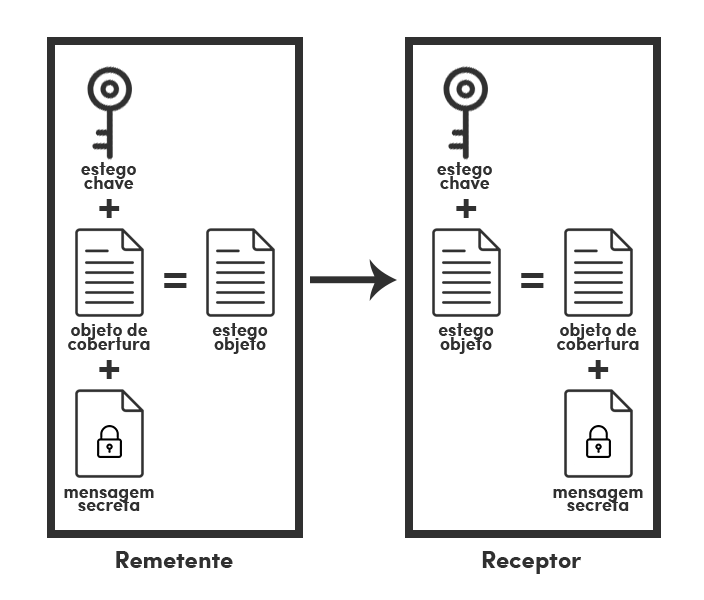
\includegraphics[width=13cm]{images/TCC1.png}
     \legend{Fonte: Imagem produzida pelo Autor}
     \label{fig_steg}
\end{figure}

\subsubsection{Tipos de Esteganografia}

Como citado anteriormente, a chave \textit{k} é opcional, sendo que sua presença e tipo podem classificar um método de esteganografia em 3 classes: esteganografia pura, esteganografia de chave privada e esteganografia de chave pública. Caso não exista uma chave, então temos uma esteganografia pura onde não há nenhuma troca de informações secretas anterior à comunicação. Apesar de possuírem implementações normalmente mais simples, métodos de esteganografia pura ferem o segundo princípio de Kerckhoffs \cite{Kerckhoffs1883}, que aconselha que a segurança de um sistema de cifragem seja baseada em uma chave e não no algoritmo de cifragem, dessa forma caso o funcionamento do sistema seja conhecido pelo atacante, ele ainda não é capaz de quebra-lo sem a chave. Por consequência disso, o recomendado é que se utilizem os métodos baseados em chaves.

 Na esteganografia de chave privada, é necessário que as duas partes compartilhem uma única chave que será utilizada durante o processo de inserção da mensagem secreta, de forma impossibilitar que qualquer atacante sem possa da chave seja capaz de decifrar a mensagem mesmo que tenha conhecimento do algoritmo. Essa classe possui conceitos que são análogos à criptografia simétrica, herdando portanto seus contratempos, sendo o principal deles a necessidade de um canal seguro para que a chave privada seja compartilhada antes do início da comunicação \cite{anderson}.

 A terceira classe de métodos é derivada da criptografia assimétrica, exigindo de um par de chaves, uma pública e uma privada. Durante o processo de inserção dos dados no objeto de cobertura, a chave pública é utilizada, enquanto para a recuperação da mensagem original é usada a chave privada. Pode-se inclusive construir um método de esteganografia de chaves públicas em cima de uma base de um sistema criptográfico de chaves públicas \cite{anderson}.

 \subsubsection{Aplicações Modernas}

 Em tempos anteriores à popularização de computadores a esteganografia possuía um leque de aplicações fortemente confinado à transmissão de mensagens secretas entre dois correspondentes. A razão disso passa primeiramente pela falta de eficiência nos métodos utilizados, e em seguida pelo fato de que as aplicações modernas que conhecemos hoje sequer eram um assunto existente na sociedade da época.
 
 O campo de marcas d´água digitais surge com a necessidade de inserir e verificar provas de autoria e propriedade de recursos digitais, e avança conforme as legislações específicas de grandes países ou blocos são sancionadas. Entretanto, nessa área os requisitos para a utilização de um algoritmo diferem dos habituais, dado que existe a necessidade de impedir que a marca seja retirada ou corrompida por transformações no arquivo. Além disso, a invisibilidade completa da mensagem nem sempre é indispensável e podemos ter marcas d'água visíveis para um observador externo. Mesmo com essas ressalvas, é notório que os últimos anos de evolução das técnicas de esteganografia foram fortemente voltados para aplicações na área de marcas d´água digitais, por seu apelo comercial latente \cite{9187785}.
 
 Apesar da natureza distinta entre as duas áreas, grande parte dos algoritmos utilizados para esteganografia podem ser transpostos para a aplicação de marcas d´água, visto que possuem a robustez necessária para impedir a mensagem de ser violada e que a ocultação da mesma não é um impeditivo \cite{9187785}. E, de fato, possuímos exemplos de usos extensivos como os micropontos invisíveis a olho nu adicionados por impressoras comerciais em suas impressões \cite{10.1145/2656434.2656437} e as câmeras digitais com capacidade de adicionar uma marca invisível em cada foto que tiram \cite{blythe}.

 \subsubsection{Problema dos Prisioneiros}

 Formulado por Simmons, o problema dos prisioneiros é um modelo utilizado para para descrever comunicação subliminar a partir de um canal monitorado. No problema os dois prisioneiros Armando e Bruna estão confinados em celas diferentes e Chico, o carcereiro, inspeciona toda a comunicação entre eles, descartando qualquer tipo de mensagem criptografada ou de conteúdo suspeito, forçando os dois a traçarem seu plano de fuga utilizando apenas comunicação invisível \cite{Simmons1984}. Podemos assumir que em um momento anterior à prisão, os dois prisioneiros combinaram uma chave a ser utilizada para algum tipo de comunicação e que o carcereiro atua de forma passiva apenas validando as mensagens sem alterá-las. Além disso, assumimos que o canal de comunicação é conhecido por Chico, para obedecer ao segundo princípio de Kerckhoffs.

 Dessa forma podemos utilizar o diagrama exposto na Figura \ref{fig_steg} para descrever uma troca de mensagens dentro do problema dos prisioneiros. Em uma cela, Armando escolhe uma mensagem inocente que será utilizada como objeto de cobertura e insere a mensagem secreta processada a partir da estego chave, gerando um estego objeto que é passado pelo canal de comunicação monitorado por Chico, e em outra cela, Bruna recebe o estego objeto e reconstrói a mensagem secreta a partir da chave combinada. Caso essa comunicação seja feita sem que o carcereiro consiga detectar a existência de uma mensagem no estego objeto podemos dizer que ela foi bem sucedida e invisível. Ao longo desse trabalho iremos utilizar esse problema de forma a buscar uma solução satisfatória para ele. 

\subsection{Arquivos Executáveis}

A esmagadora maioria das pessoas programadoras atualmente escreve código em linguagens de alto nível que são muito próximas de línguas humanas, enquanto computadores modernos interpretam sequências de instruções representadas em base binária. Isso só é possível graças a compiladores, softwares que transformam construções feitas em linguagens de alto nível para o que chamamos de linguagem de máquina \cite{patterson}.

O processo de compilação usualmente toma como parâmetros de inicialização um código fonte escrito em uma linguagem de alto nível e produz um arquivo, comumente chamado de arquivo executável. Esse arquivo é capaz de ser carregado para o processador e executar as instruções dadas pelo programa. Esses arquivos podem possuir estruturas e formatos diferentes, dependendo do sistema operacional e do processador alvos que foram usados. Atualmente os dois formatos mais utilizados são o ELF e PE, utilizados respectivamente pelos sistemas operacionais Linux \cite{linuxbase_4} e Windows \cite{microsoft_pe}. Apesar de possuirem diferenças, ambos os formatos citados compartilham características. Além do código já devidamente representado em linguagem de máquina, os arquivos carregam um cabeçalho com metadados referentes ao programa.

\subsubsection{ELF (\textit{Executable and Linkable Format})}

O formato ELF foi desenvolvido inicialmente pela Unix System Laboratories em 1988, ganhando notoriedade e implementações em outros sistemas, até que em 1999 foi adotado como padrão pelo sistema Unix e seus derivados. Por ser facilmente generalizado para diversos tipos de sistemas e possuir suporte para a maioria das funcionalidades utilizadas pela indústria atualmente, continua até hoje figurando entre os formatos mais relevantes para arquivos executáveis.

Estruturalmente, um arquivo ELF é dividido em duas estruturas principais: segmentos e seções. Os segmentos contém informações úteis para o programa durante seu tempo de execução, como o local e valores de constantes definidas em código e as próprias instruções do programa. As seções possuem dados utilizados em tempo de ligação ou para \textit{debugging} como símbolos gerados no processo de compilação e endereços de realocação de memória \cite{elf}.

Para organizar essas informações, é utilizado um esquema de cabeçalhos contendo metadados e posições dos segmentos e seções. Logo no início do arquivo está o \textit{ELF Header} detalhando informações como arquitetura alvo, tipo de arquivo e posições para os próximos cabeçalhos. Em seguida começam os \textit{Program Headers} que definem como estão dispostos os segmentos no arquivo, os próprios segmentos e seções com seus conteúdos e por fim os \textit{Section Headers} contendo as informações das seções. A estrutura típica de um executável contendo código e dados pode ser vista na figura a seguir, notando que é comum essa sobreposição entre secções e segmentos na memória \cite{elf}.

\begin{figure}[!htb]
     \centering
     \caption{Estrutura de um arquivo ELF contendo dados e código.}
     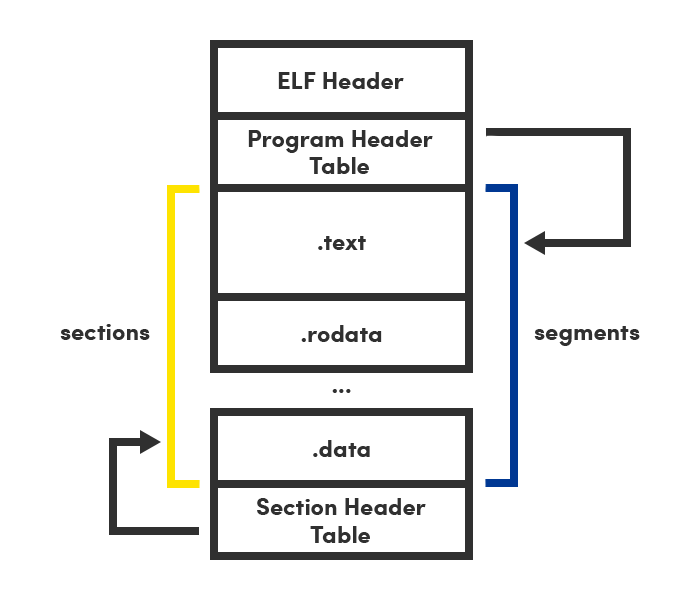
\includegraphics[width=13cm]{images/TCC2.png}
     \legend{Autor: Imagem produzida pelo Autor}
     \label{}
\end{figure}

\subsection{Arquitetura RISC-V}

Assim como nem todos os humanos compreendem a mesma língua, nem todas as máquinas sabem interpretar a mesma linguagem. Existem diversas formas de representar a linguagem de máquina desenvolvidas ao passar das décadas por diferentes fabricantes de computadores, cada máquina possuindo seu próprio conjunto de instruções que é capaz de executar. Esse conjunto é comumente denominado \textit{Instruction Set Architecture} (ISA) e todas as máquinas que compreendem um mesmo conjunto são ditas da mesma arquitetura.

Atualmente duas grandes filosofias de construção de arquiteturas disputam espaço no mercado, \textit{Complex Instruction Set Computer} (CISC) e \textit{Reduced Instruction Set Computer} (RISC), tendo como mote principal a complexidade do seu conjunto de instruções. Enquanto máquinas CISC possuem um conjunto de instruções maior e essas instruções também contém um grau de complexidade mais elevado, as máquinas RISC possuem poucas operações e buscam realizar as operações de forma fragmentada em uma quantidade maior de passos simples \cite{patterson_risc_i}.

Em consequência dos princípios básicos de cada tipo de máquina, é possível inferir características que serão comuns a todas as arquiteturas de cada classe. Máquinas CISC costumam gerar códigos menores, pois aglutinam diversas operações em uma só instrução, enquanto nas implementações RISC temos o oposto. Entretanto, apesar da quantidade total de instruções geradas para um mesmo código na máquina RISC ser maior, cada instrução possui uma execução mais rápida devido a sua simplicidade, retomando de volta a performance perdida por executar um número maior de instruções \cite{patterson_risc_i}.

Nos dias atuais a melhor representação de uma arquitetura CISC é a x86, desenvolvida inicialmente pela Intel em 1978 como uma extensão da arquitetura 8080. Apesar de ser coloquialmente referida como uma arquitetura, é na verdade um conjunto que abarca diversas ISAs desenvolvidas ao longo das décadas. Para máquinas RISC podem ser citadas as arquiteturas \textit{Advanced RISC Machine} (ARM) e RISC-V, sendo que a última possui esse nome por ser a quinta geração de arquiteturas RISC a ser desenvolvida pela Universidade da Califórnia.

A arquitetura RISC-V é uma ISA desenvolvida de forma aberta e sem cobrança de \textit{royalties}, originalmente pelo departamento de engenharia elétrica e ciências da computação da Universidade da Califórnia, campus Berkeley. Entretanto, desde o início em 2010 até o presente, muitos contribuidores externos, independentes ou em contribuições corporativas, participaram do projeto. Diferentemente do usual para projetos acadêmicos, o RISC-V busca não apenas ser um objeto de estudo teórico, mas também ter viabilidade para projetos reais na indústria \cite{Asanović:EECS-2014-146}.

O RISC-V possui um conjunto de apenas 47 instruções obrigatórias, complementadas por extensões padronizadas de propósitos gerais que adicionam funcionalidades como multiplicação, operações atômicas e aritmética de ponto flutuante. Todas as operações são realizadas exclusivamente em registradores, utilizando o conceito de \textit{load/store machine}, para operar sobre um valor em memória primeiro é necessário uma instrução para carregá-lo em um registrador, em seguida é realizada a operação em uma segunda instrução, e por fim uma última instrução retorna o valor para a memória \cite{Waterman:EECS-2014-54}.

Seguindo princípios da filosofia RISC e utilizando erros de experiências passadas para aprimorar o novo projeto, atualmente o RISC-V é considerado por grande parte da comunidade como o futuro do \textit{hardware open source}, possibilitando que universidades, indivíduos e empresas possam criar implementações completamente livres em cima de uma base sólida.

\section{Trabalhos Relacionados}

Apesar de não ser um assunto extensamente explorado, a esteganografia utilizando código executável já foi proposta e estudada por outros autores ao longo dos últimas décadas.
O projeto Hydan utiliza instruções semânticamente equivalentes como decisores binários para inserir dados dentro de um código executável para a arquitetura x86. Entretanto, a razão de codificação de em média 1 bit de mensagem para cada 100 bits do objeto de cobertura encontrada é insatisfatória para alguns casos de uso \cite{Hydan}. No mesmo ano, Anckaert \textit{et al} (2004) expandem o conceito inicial do Hydan, realizando um estudo sobre a redundância em programas da arquitetura x86 e formulando critérios de substituição claros. Além disso, esse trabalho também traz um \textit{framework} para análise de detectabilidade dos estego-objetos gerados.

O \textit{whitepaper} publicado por Wright (2008) desenvolve em cima de um tópico já citado pelos autores originais do Hydan: a fragilidade do trabalho em relação a detectabilidade. O método aplicado pelos pesquisadores não leva em consideração a distribuição estatística das instruções em cada plataforma, permitindo que uma análise seja feita buscando anomalias, comparando instruções contidas no programa alvo com a distribuição normalmente encontrada em programas compilados para a mesma plataforma \cite{Wright2020DetectingHS}.

Outra abordagem foi tomada por Shin \textit{et al} (2008), que desenvolve um método para inserção de dados em arquivos do formato PE, adicionando os dados na seção \textit{.text} do binário e tomando providências de realocação caso seja necessário. Apesar desse método possuir uma flexibilidade maior e capacidade de codificação virtualmente infinita, ele altera o tamanho do arquivo em disco, portanto pode ser detectado por um observador externo em posse do objeto de cobertura, invalidando essa técnica para aplicações em que o arquivo original seja de alguma forma público. De forma complementar, um trabalho posterior propõe um método similar cobrindo as mesmas plataformas e adicionando uma camada de criptografia \cite{zaidan}.

Além de métodos diferentes para a inserção dos dados no objeto de cobertura, a natureza dos próprios dados é espaço de pesquisas. Lu, Xiong e Gao (2014) elaboraram a ideia de utilizar esteganografia não só para esconder uma mensagem dentro de um código fonte, mas sim para esconder parte do código fonte dentro de si mesmo. Os autores utilizam \textit{Return Oriented Programming} (ROP) em combinação com esteganografia para que certos conjuntos de instrução sejam invisíveis à analisadores estáticos de código mas ainda sejam executadas em tempo de execução. Como prova de conceito é apresentada a ferramenta RopSteg que utiliza uma versão modificada do algoritmo de \textit{Galileo} para gerar segmentos de código contendo estruturas de retorno que não estavam no binário original. Entretanto, apesar de conseguirem êxito para fazer as alterações no arquivo, devido à ROP ser frequentemente associada com malwares, os autores alertam que existe a possibilidade do arquivo gerado ser marcado como malicioso por sistemas de detecção \cite{ropsteg}.

Por fim, existem ainda implementações não acadêmicas porém relevantes, utilizando propostas levantadas pelos autores anteriores e que de certa formam fornecem alguma validação da viabilidade material desses métodos. A ferramenta \textit{steg86} apropria-se da ideia inicial dos autores do Hydan para desenvolver uma interface de linha de comando simples para ocultação de dados em binários compilados para as plataformas x86 e AMD64, oferecendo suporte tanto para ELF quanto para PE. Além de operações básicas de injeção e extração de mensagens, o utilitário também oferece um comando para fazer uma análise de um binário e determinar quantos bits podem ser inseridos nele \cite{steg86}.
% ---

% ---
% 3 - Desenvolvimento da técnica
% ---
% ----------------------------------------------------------
\chapter{Desenvolvimento da Técnica}\label{cap:desenvolvimento}

Durante esse capítulo serão detalhadas as técnicas e passos utilizados para atingir os objetivos citados no Capítulo 1, iniciando com o desenvolvimento de ferramentas de apoio, experimentos com a aplicação de métodos esteganográficos existentes na ISA do RISC-V e a execução do projeto em uma aplicação de linha de comando de uso geral.

Ao longo deste capítulo serão introduzidos conceitos necessários para a compreensão do algoritmo proposto como objetivo, com uma pesquisa calcada tanto em materiais e documentos históricos quanto produções acadêmicas recentes de maior relevância.

\subsection{Aplicações para Experimentos e Validações}

Para avaliar os resultados obtidos pelas técnicas de esteganografia e validar o ferramental de apoio desenvolvido durante este trabalho foram utilizado dois conjuntos de classes distintas de programas como objetos de experimento. O primeiro conjunto contém a compilação de 2 sistemas operacionais, o segundo conjunto é composto 22 programas utilitários de bancos de dados. Os sistemas operacionais foram selecionados devido a alta gama de operações distintas realizadas por esse tipo de programa durante sua execução. Os utilitários com enfoque para bancos de dados foram escolhidos por possuirem em seu código algoritmos variados de ordenação, busca e transformação de dados, com o intuito de entender se um programa altamente focado em operações em disco é mais suscetível a técnicas de esteganografia. 

Para ambos os conjuntos de programas foi utilizado o processo de compilação cruzada a partir de uma máquina x86 tendo como arquitetura alvo o RISC-V para eliminar a necessidade de possuir uma placa física implementando RISC-V. No primeiro conjunto os softwares utilizados foram o EPOS (Embedded Parallel Operating System), desenvolvido com o propósito de ser um SO enxuto e eficiente capaz de ser executado em microprocessadores de sistemas embarcados e o Linux, um SO de propósito geral utilizado na maioria dos dispositivos pelo mundo e que conta com funcionalidades mais variadas e robustas do que o primeiro. Para o segundo conjunto foram utilizados os utilitários gerados na compilação do SGBD PostgreSQL, que incluem o próprio SGBD e outros módulos utilizados para funcionalidades específicas do software. As Tabelas \ref{tab:prog_1} e \ref{tab:prog_2} contém os nomes, versões e tamanhos de arquivos (descritos em bits) de todos os softwares utilizados para os experimentos, separados em seus conjuntos. 

\begin{table}[htb]
    \centering
    
    \begin{tabular}{|c|c|c|}
        \hline
        Programa & Versão  & Tamanho\\
        \hline
        Linux & v6.5 & 150792320 \\
        \hline
        EPOS & v2.2.2 & 288128 \\
        \hline
    \end{tabular}
    \caption{Conjunto 1 de programas utilizados nos experimentos}
    \label{tab:prog_1}
\end{table}

\begin{table}[htb]
    \centering
    
    \begin{tabular}{|c|c|c|}
        \hline
        Programa & Versão  & Tamanho\\
        \hline
        initdb & v16.0.0 & 1252608 \\
        \hline
        pgbench & v16.0.0 & 1502784 \\
        \hline
        pg\_amcheck & v16.0.0 & 809536 \\
        \hline
        pg\_archivecleanup & v16.0.0 & 372736 \\
        \hline
        pg\_basebackup & v16.0.0 & 1197632 \\
        \hline
        pg\_checksums & v16.0.0 & 657152 \\
        \hline
        pg\_config & v16.0.0 & 360512 \\
        \hline
        pg\_controldata & v16.0.0 & 475456 \\
        \hline
        pg\_ctl & v16.0.0 & 566784 \\
        \hline
        pg\_dump & v16.0.0 & 2857344 \\
        \hline
        pg\_dumpall & v16.0.0 & 1003264 \\
        \hline
        pg\_receivewal & v16.0.0 & 876736 \\
        \hline
        pg\_recvlogical & v16.0.0 & 841408 \\
        \hline
        pg\_resetwal & v16.0.0 & 524928 \\
        \hline
        pg\_restore & v16.0.0 & 1414208 \\
        \hline
        pg\_rewind & v16.0.0 & 1252928 \\
        \hline
        pg\_test\_fsync & v16.0.0 & 405504 \\
        \hline
        pg\_test\_timing & v16.0.0 & 331136 \\
        \hline
        pg\_upgrade & v16.0.0 & 1247936 \\
        \hline
        pg\_verifybackup & v16.0.0 & 864768 \\
        \hline
        pg\_waldump & v16.0.0 & 843392 \\
        \hline
        psql & v16.0.0 & 3672768 \\
        \hline
    \end{tabular}
    \caption{Conjunto 2 de programas utilizados nos experimentos}
    \label{tab:prog_2}
\end{table}
\section{Ferramental de Suporte}

A fim de alcançar os objetivos propostos por este trabalho foi necessário estudar tópicos satélites e desenvolver aplicações utilitárias quando não houvessem projetos \texttt{open source} capazes de suprir a necessidade. Essas aplicações estão distribuídas no formato de módulos Python e podem ser usadas de forma independente.

\subsection{\textit{Parser} para arquivos ELF}

A partir da decisão de trabalhar diretamente em arquivos binários modificando sua estrutura e conteúdo base com o intuito de esconder informações se cria a necessidade de poder abrir, interpretar, analisar e editar arquivos no formato de escolha. Como definido no capítulo passado, este trabalho foca em explorar o formato ELF utilizado amplamente em sistemas Unix. Apesar da existência de utilitários capazes de executar essa tarefa a decisão por desenvolver o \textit{parser} dentro projeto foi tomada pela facilidade em analisar apenas as informações estritamente necessárias para encontrar trechos de instruções de máquina dentro do arquivo, otimizando a performance geral do código.

O funcionamento do \textit{parser} é baseado na leitura de cabeçalhos contendo as informações sobre as seções e segmentos de um arquivo ELF, codificados de forma numérica correspondente a tabelas definidas na especificação do formato. Primeiramente fazemos a leitura do \textit{ELF Header} para nos certificarmos de que o arquivo foi compilado para a arquitetura RISC-V e extraímos informações importantes para os próximos passos, como a ordenação dos \textit{bytes}, o número de seções e segmentos e o índice da tabela de símbolos. Para os objetivos da aplicação desenvolvida, os segmentos serão ignoradas pelo algoritmo, utilizando apenas seções para encontrar porções de código.

Em seguida fazemos a leitura sequencial dos cabeçalhos de seções, utilizando os dados sobre permissões e tipo para identificar trechos de código no arquivo. Ao encontrar uma seção de código é possível pular para seu endereço relativo e retornar os blocos de 32 \textit{bits} correspondentes às instruções de máquina contidas no código. Esse passo do algoritmo é realizado até que a seção seja esgotada, ao ponto em que será buscada a próxima seção para que se repitam os passos anteriores até o esgotamento do próprio arquivo. Com esse processo finalizado temos a lista completa de instruções contidas no programa e já é possível manipulá-las.

% TODO: colocar um diagrama do parser

\subsection{Decodificador e Codificador  para instruções RISC-V}

Após a extração completa de todas as instruções presentes em um binário resta apenas uma longa lista de números com 32 \textit{bits} sem um significado claro para um leitor humano. Para que qualquer técnica esteganográfica seja aplicada sobre uma mídia digital é necessário compreender a semântica dos dados, de modo a evitar o corrompimento acidental da informação contida. Com o propósito de decodificar as instruções para um formato mais legível por seres humanos foi desenvolvido um decodificador de instruções capaz de receber um objeto \textit{bytes} e retornar a instrução correspondente escrita em Assembly.

A especificação do RISC-V introduz conjuntos de instruções base e extensões de propósitos específicos com suas próprias instruções que evoluem com o passar das versões da plataforma, obedecendo formatos de codificação de instruções que definem a posição e semântica dos campos dentro dos 32 bits disponíveis. O conjunto base contém 6 formatos definidos capazes de codificar as instruções mais básicas para o funcionamento de um processador RISC-V, esses formatos estão descritos nas especificações técnicas da arquitetura \cite{riscv_manual_vol1}. 

\begin{figure}[!htb]
     \centering
     \caption{Formatos de Instrução disponíveis na ISA base do RISC-V.}
     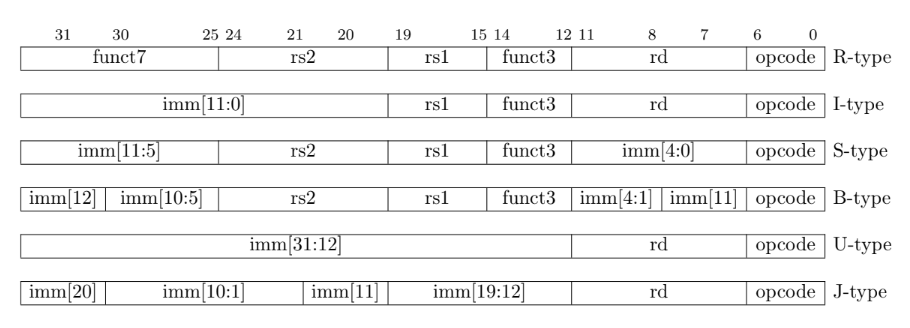
\includegraphics[width=13cm]{images/TCC3.png}
     \legend{Autor: Retirado de \cite{riscv_manual_vol1}}
     \label{}
\end{figure}

Para os propósitos desejados nessa implementação cobrir estes 6 tipos é suficiente, dado que formatos específicos de extensões são menos comuns em programas compilados e podem variar conforme os processadores que adotam a arquitetura. O processo de decodificação foi realizado de forma a identificar inicialmente a qual formato uma instrução pertence utilizando o campo \textit{opcode} que compreende os 7 primeiros bits de cada conjunto de 32 bits gerados pelo compilador. Após a identificação do formato, os demais campos são separados utilizando operações binárias, respeitando particularidades de campos com sinal aritmético para valores numéricos e consultando as tabelas de operações descritas na especificação da ISA. Com todos os campos já traduzidos a instrução é montada em Assembly já com seu mnemônico, registradores e operandos identificados. 

Após a decodificação é criado também um objeto editável contendo os campos de cada instrução para que seja possível alterar os valores representados em alto nível, expondo um método capaz de realizar a transformação reversa, utilizando os campos da instrução para gerar sua contraparte binária. Dessa forma, uma instrução pode ser decodificada, alterada e então recodificada de volta para seu formato binário, podendo ser sobrescrita no arquivo fonte. Esse processo em conjunto com o \textit{parser} de arquivos ELF permite a livre manipulação de qualquer instrução presente em um binário compilado para RISC-V e é a base utilizada posteriormente pelo algoritmo esteganográfico para inserir dados na mídia de destino.

A implementação do decodificador e codificador foi baseada no trabalho de pesquisadores da Universidade de Columbia, desenvolvido na linguagem Javascript com propósitos educacionais \cite{rvcodec}. O projeto \textit{rvcodec.js} visa facilitar o ensino da ISA disponibilizando uma ferramenta online para conversão de instruções e cobre as principais extensões da plataforma além do conjunto base.

\subsubsection{Experimento de Validação}

Os dois conjuntos de testes foram utilizados como método de avaliação da capacidade de decodificação do módulo apresentado, utilizando como métrica a razão entre a quantidade de instruções presentes no programa e a quantidade de instruções que foram decodificadas após o processo. O esperado desse experimento era verificar se os 6 formatos de instrução da ISA base cobrem uma porção suficientemente grande de um binário arbitrário para que seja possível obter taxas de codificação satisfatórias posteriormente. Analisando resultados do experimento presentes nas Tabelas 2 e 3 pode-se notar que a cobertura da ISA base ocupa altas taxas dentro das seções de código do programa, o que indica o potencial para níveis sólidos de codificação de informação apenas com instruções desses formatos.

\begin{table}[!h]
    \centering
    
    \begin{tabular}{|c|c|}
        \hline
        Programa & Percentual de Instruções Decodificadas \\
        \hline
        Linux & 63.55\% \\
        \hline
        EPOS & 70.63\% \\
        \hline
    \end{tabular}
    \caption{Resultados do Experimento do Decodificador para o Conjunto 1}
    \label{tab:exp1_1}
\end{table}

\begin{table}[!h]
    \centering
    
    \begin{tabular}{|c|c|}
        \hline
        Programa & Percentual de Instruções Decodificadas \\
        \hline
        initdb & 76.25\% \\
        \hline
        pgbench & 66.07\% \\
        \hline
        pg\_amcheck & 61.71\% \\
        \hline
        pg\_archivecleanup & 64.58\% \\
        \hline
        pg\_basebackup & 68.58\% \\
        \hline
        pg\_checksums & 63.47\% \\
        \hline
        pg\_config & 67.76\% \\
        \hline
        pg\_controldata & 65.86\% \\
        \hline
        pg\_ctl & 68.65\% \\
        \hline
        pg\_dump & 68.77\% \\
        \hline
        pg\_dumpall & 75.62\% \\
        \hline
        pg\_receivewal & 63.36\% \\
        \hline
        pg\_recvlogical & 64.32\% \\
        \hline
        pg\_resetwal & 65.45\% \\
        \hline
        pg\_restore & 68.59\% \\
        \hline
        pg\_rewind & 66.74\% \\
        \hline
        pg\_test\_fsync & 61.10\% \\
        \hline
        pg\_test\_timing & 65.93\% \\
        \hline
        pg\_upgrade & 76.21\% \\
        \hline
        pg\_verifybackup & 61.90\% \\
        \hline
        pg\_waldump & 63.22\% \\
        \hline
        psql & 69.99\% \\
        \hline
    \end{tabular}
    \caption{Resultados do Experimento do Decodificador para o Conjunto 2}
    \label{tab:exp1_2}
\end{table}

\section{Aplicação de Técnicas Conhecidas}
% ----------------------------------------------------------
Nessa seção está descrito todo o processo, análise e aplicação de técnicas já conhecidas na litetura para codificação de informação em arquivos binários, a fim de verificar sua viabilidade quando transpostas para a arquitetura RISC-V. Foram analisadas apenas técnicas cuja aplicação não envolvem alteração do tamanho do arquivo final ou realocação de endereços ou etiquetas, de forma a manter a viabilidade da implementação para uma gama maior de casos de uso.

\subsection{Alocação de Registradores}

A especificação atual da arquitetura RISC-V prevê 32 registradores de 32 bits para serem utilizados com valores inteiros e outros 32 registradores disponíveis para valores de ponto flutuante, sendo que apenas 8 registradores em cada um desses conjuntos é reservado para alocação de argumentos. Apesar de teoricamente ser possível codificar bits utilizando a escolha dos registradores alocados para cada chamada de função, a convenção de chamadas prevê que esses registradores sejam escolhidos de forma ordenada e crescente, impedindo o uso prático dessa abordagem para implementações \cite{riscv_manual_psabi}.

\subsection{Escalonamento de Instruções}

Certas operações de alto nível quando executadas pelo processador passam por um desmembramento em duas ou mais instruções nativas que podem ser independentes entre si, gerando uma decisão de ordenação que pode ser explorada com o intuito de codificar bits de informação. Tal técnica foi utilizada por Anckaert \textit{et al} (2004) com a arquitetura alvo sendo IA-32, uma arquitetura CISC que dispõe de um número elevado de instruções redundantes ou semelhantes que podem performar operações equivalentes, portanto seus resultados são satisfatórios.

Entretanto, quando o contexto é alterado para uma arquitetura RISC o número de permutações equivalentes a  cada operação de alto nível tende a ser reduzido, impactando na eficiência desse método. Além disso o esforço necessário a ser empregado para essa técnica também é custoso pois requer a implementação de uma ferramenta capaz de gerar todas as permutações possíveis para cada procedimento a que se deseje explorar. A partir do entendimento de que esse método possui um alto custo temporal de implementação e a expectativa de resultados é baixa, o escalonamento de instruções não será abordado durante a execução desse trabalho.

\subsection{Substituição de Instruções Equivalentes}

A estratégia de utilizar escolhas dentro de uma única instrução como estrutura de codificação binária é amplamente utilizada por autores desde os primeiros trabalhos realizados na área, El-Khalil e Keromytis (2004) baseiam sua solução em criar tabelas de instruções equivalentes e atribuir um valor para cada alternativa, dessa forma para cada instrução pertencente a um conjunto de instruções equivalentes, podemos codificar log2(n) bits, sendo n o tamanho do conjunto. Os autores catalogaram 18 conjuntos de equivalência dentro da ISA \texttt{x86}, variando entre operações aritméticas e binárias, com equivalências produzidas por ordem de operandos e inversas matemáticas de instruções.

Devido as diferenças filosóficas entre arquiteturas RISC e CISC, a aplicação direta dessa técnica possui uma eficiência reduzida, com um número menor de conjuntos equivalentes a serem explorados por um algoritmo de substituição. Muitas das redundâncias comuns em outras ISAs foram removidas propositalmente durante o desenvolvimento do RISC-V, restando apenas aquelas que seriam impossíveis de remover como as equivalências lógicas e aritméticas axiomáticas. Após analisar o conjunto base de instruções foram obtidos 5 grupos contendo exatamente 2 instruções cada, o que permite a codificação de 1 bit por cada instrução pertencente ao grupo.

\begin{table}[!htb]
    \centering
    
    \begin{tabular}{|c|c|}
        \hline
        Nome do grupo & Instrução  \\
        \hline
        \hline
        add-group & add rd, rs1, rs2 \\
                  \hline
                  & add rd, rs2, rs1 \\
        \hline
        and-group & and, rd, rs1, rs2 \\
                  \hline
                  & and, rd, rs2, rs1 \\
        \hline
        or-group & or, rd, rs1, rs2 \\
                  \hline
                  & or, rd, rs2, rs1 \\
        \hline
        beq-group & beq, rd, rs1, rs2 \\
                  \hline
                  & beq, rd, rs2, rs1 \\
        \hline
        bne-group & bne, rd, rs1, rs2 \\
                  \hline
                  & bne, rd, rs2, rs1 \\
        \hline
    \end{tabular}
    \caption{Conjuntos de instruções equivalentes no RISC-V}
    \label{tab:equiv_sets}
\end{table}

Ao examinar todas as instruções encontradas nota-se que as equivalências são puramente baseadas na comutatividade de operações lógicas e aritméticas. As instruções encontradas são operações comuns e presentes em todo programa de computador, o que indica uma possível abundância de espaço para codificação de informação. Ademais, não existe uma convenção da arquitetura que denote qual deva ser a ordem dos operandos de uma determinada instrução, dessa forma podemos descrever o passo a passo para codificar bits utilizando essa estratégia utilizando o Algoritmo 1.

%% This declares a command \Comment
%% The argument will be surrounded by /* ... */
\SetKwComment{Comment}{/* }{ */}
\SetKw{Kw}{continue}
\begin{algorithm}
    \caption{Codificação de bits utilizando substituição de instruções equivalentes}\label{alg:one}
    $P \gets \{...\}$\;
    \BlankLine
    $I \gets \{...\}$\;
    \BlankLine
    $M \gets "01000110010011000100000100000000"$\;
    \BlankLine
    $message\_index \gets 0$;
    \BlankLine
    \While{$message\_index$ <= \|$M$\|}{
        $encoded \gets false$\;
        
        \While{$encoded$ == $false$}{
            \BlankLine
            $instruction$ \gets next($P$)\;
            \BlankLine
    
            \If{$instruction$ not in $I$}{
                \Kw{}\;
            }
    
            \BlankLine
                
            \If{$instruction$.rs1 == $instruction$.rs2}{
                \Kw{}\;
            }
            \BlankLine
            
            \eIf {$char$ == "1"} {
                \If{not ($instruction$.rs1 > $instruction$.rs2)}{
                    swap($instruction$.rs1, $instruction$.rs2)\;
                }
            } {
                \If{not ($instruction$.rs1 < $instruction$.rs2)}{
                    swap($instruction$.rs1, $instruction$.rs2)\;
                }
            }
            \BlankLine
            $encoded \gets true$\;
        }
    }
\Return $P$\;
\end{algorithm}

Inicialmente define-se \textit{P} como o conjunto contendo todas as instruções do programa alvo ordenadas pelo seu endereço relativo ao arquivo, \textit{I} como o conjunto de instruções capazes de codificar um bit (vistos na Tabela 2) e \textit{M} como a mensagem binária a ser inserida no arquivo, foi definido que para esta implementação o critério de final da mensagem é dado por um caractere ASCII nulo, representado por 8 bits de valor zero. Em seguida itera-se por cada caractere da mensagem buscando a próxima instrução que esteja contida em \textit{I}. Ao encontrar uma instrução candidata, caso seus dois operandos sejam idênticos é necessário buscar outra pois é impossível codificar uma escolha nessa situação. Do contrário, é possível codificar um bit ordenando os operandos de acordo com um critério pré estabelecido, durante a execução deste trabalho usaremos como critério a função $\mathit{f}$ definida por:

\begin{equation}
    f(rs1, rs2) =
    \begin{cases*}
      1 & se $rs1 > \mathit{rs2}$ \\
      0 & se $rs2 > \mathit{rs1}$ \\
      \phi        & caso contrário
    \end{cases*}
\end{equation}

Ao final da iteração pelos caracteres da mensagem o conjunto \textit{P} representa a lista de instruções já com a mensagem embutida em si, a partir desse ponto o codificador RISC-V pode aplicar o processo reverso para transformar as instruções em linguagem de montagem para código de máquina e escrever o arquivo final que representa o estego-objeto. Otimizações ainda podem ser feitas no algoritmo apresentado a fim de minimizar laços de repetição, reduzir uso de memória da aplicação e número escritas ao arquivo e serão expostas em um próximo capítulo.

Para decodificar uma mensagem propõe-se um algoritmo semelhante ao anterior, tomando \textit{P} como o conjunto de todas as instruções do programa, \textit{I} como o conjunto de instruções codificáveis e \textit{M} como uma \textit{string} vazia que ao final da execução receberá a mensagem decodificada. Entretanto, após encontrar uma instrução candidata para a técnica um bit é extraído a partir da ordem de seus operandos e a concatenação final de todos os bits contém a mensagem, respeitando o critério de parada de caractere nulo controlado por uma variável que é verificada a cada 8 bits para uma representação em ASCII.

\begin{algorithm}
    \caption{Decodificação de bits utilizando substituição de instruções equivalentes}\label{alg:two}
    $P \gets \{...\}$\;
    \BlankLine
    $I \gets \{...\}$\;
    \BlankLine
    $M \gets$\ string()\;
    \BlankLine
    $last\_char \gets$ string() \;
    \BlankLine
    \While{$last\_char$ != $"00000000"$} {
        \If{$last\_char$.length == $8$ }{
            $last\_char \gets $ string() \;
        }
        
        \BlankLine
        $instruction \gets$ next($P$)\;
        \BlankLine

        \If{$instruction$ not in $I$}{
            \Kw{}\;
        }

        \BlankLine
            
        \If{$instruction$.rs1 == $instruction$.rs2}{
            \Kw{}\;
        }
        
        \BlankLine

        \eIf {$instruction$.rs1 > $instruction$.rs2} {
            $M$ += $"1"$\; 
        } {
            $M$ += $"0"$\; 
        }
    }
\BlankLine
\Return $M$\;
\end{algorithm}

\subsubsection{Experimento de Validação}

Após a elaboração do algoritmo apresentado para codificação utilizando substituição de instruções equivalentes foi realizado um experimento com a motivação de examinar a quantidade de bits que poderiam ser codificados dentro de cada arquivo presente no conjunto de testes. Para isso uma pequena modificação foi realizada no algoritmo, incrementando um contador sempre que encontrada uma instrução explorável pela técnica de modo a obter no final o total de bits codificáveis. Observando os resultados expostos nas Tabela 4 e 5 é possível verificar que a técnica possui uma capacidade de codificação baixa quando comparada com os resultados obtidos para a arquitetura x86 por outros autores. A taxa de codificação média obtida por essa implementação foi de 0,03\%, inferior aos 0,9\% demonstrados por El-Khalil e Keromytis (2004) e os 3,7\% apresentados por Anckaert \textit{et al} (2004). Os resultados inferiores para a arquitetura alvo desse trabalho são explicados principalmente pelo tamanho dos conjuntos de substituições disponíveis, enquanto a arquitetura da Intel conta com 18 conjuntos contendo entre 2 a 5 instruções, o RISC-V apresenta apenas 5 conjuntos de 2 instruções cada, reduzindo tanto a frequência de aparição de instruções exploráveis no programa quanto a quantidade de bits codificados por instrução. 

\begin{table}[htb]
    \centering
    
    \begin{tabular}{|c|c|}
        \hline
        Programa & Porcentagem Codificável \\
        \hline
        Linux & 0.05\% \\
        \hline
        EPOS & 0.03\% \\
        \hline
    \end{tabular}
    \caption{Resultados do Experimento Para o Conjunto 1}
    \label{tab:exp2_1}
\end{table}

\begin{table}[htb]
    \centering
    
    \begin{tabular}{|c|c|}
        \hline
        Programa & Porcentagem Codificável \\
        \hline
        initdb & 0.02\% \\
        \hline
        pgbench & 0.03\% \\
        \hline
        pg\_amcheck & 0.02\% \\
        \hline
        pg\_archivecleanup & 0.02\% \\
        \hline
        pg\_basebackup & 0.04\% \\
        \hline
        pg\_checksums & 0.02\% \\
        \hline
        pg\_config & 0.02\% \\
        \hline
        pg\_controldata & 0.01\% \\
        \hline
        pg\_ctl & 0.02\% \\
        \hline
        pg\_dump & 0.03\% \\
        \hline
        pg\_dumpall & 0.03\% \\
        \hline
        pg\_receivewal & 0.03\% \\
        \hline
        pg\_recvlogical & 0.03\% \\
        \hline
        pg\_resetwal & 0.02\% \\
        \hline
        pg\_restore & 0.05\% \\
        \hline
        pg\_rewind & 0.03\% \\
        \hline
        pg\_test\_fsync & 0.02\% \\
        \hline
        pg\_test\_timing & 0.03\% \\
        \hline
        pg\_upgrade & 0.02\% \\
        \hline
        pg\_verifybackup & 0.04\% \\
        \hline
        pg\_waldump & 0.04\% \\
        \hline
        psql & 0.04\% \\
        \hline
    \end{tabular}
    \caption{Resultados do Experimento Para o Conjunto 2}
    \label{tab:exp2_2}
\end{table}

Entretanto, apesar de não apresentar resultados satisfatórios para codificação de grandes quantidades de dados o experimento comprova a viabilidade do uso dessa técnica para inserção de uma quantidade reduzida de bits, possibilitando o uso do método para aplicações específicas que não tenham como requisito o uso de mensagens extensas. Dado que as outras técnicas exploradas não produziram resultados por particularidades da arquitetura, a aplicação desenvolvida por esse trabalho teve como foco a utilização da substituição de instruções equivalentes como mecanismo de codificação de dados.
% ---

% ---
% 4 - Desenvolvimento da aplicação
% ---
%\phantompart
% ----------------------------------------------------------
\chapter{Desenvolvimento da Aplicação}
% ----------------------------------------------------------

Na extensão deste capítulo serão abordadas as técnicas, decisões de projeto e desenvolvimento da aplicação proposta nos objetivos do trabalho, implementando o método descrito no Capítulo 3 como estrutura de codificação de dados e apresentando um \textit{software} capaz de inserir uma mensagem arbitrária dentro de um arquivo binário de código compilado.

\section{Escolha de Linguagem e Definições Gerais do Projeto}

\subsection{Linguagem e Ambiente}

Para todos os desenvolvimentos práticos foi definido o uso da linguagem Python, conhecida por sua simplicidade e clareza de código, o que facilita a compreensão para os pesquisadores e desenvolvedores de diversas áreas, em sua versão 3.10. Além disso, a vasta gama de bibliotecas e módulos disponíveis em Python, como \texttt{struct}, \texttt{pickle}, e \texttt{array}, oferece funcionalidades prontas para o tratamento de dados binários, economizando tempo e esforço no desenvolvimento. A portabilidade do Python também é uma vantagem, já que a linguagem é suportada em diferentes sistemas operacionais, garantindo que os resultados do projeto sejam facilmente reproduzíveis. Por fim, a comunidade Python ativa e os recursos de documentação tornam mais simples a resolução de problemas e o suporte durante o desenvolvimento do projeto.

Até o momento da publicação dessa monografia não existe uma forma obrigatória definida pela linguagem de como estruturar seus projetos, portanto foram seguidas as recomendações dadas no livro \textit{The Hitchhiker's Guide to Python} que são utilizadas em larga escala pela comunidade \cite{reitz2016hitchhiker} em conjunto com o gerenciador de dependências Poetry utilizado para distribuir de forma homogênea a aplicação em diversas máquinas \cite{poetry}.

\subsection{Estrutura de módulos}

A aplicação está organizada em módulos Python com responsabilidades distintas a fim de hermetizar cada funcionalidade em um único local e evitar dependências desnecessárias e facilitar a manutenabilidade de cada módulo. Em seguida estão descritos os módulos com relevância para o entendimento da implementação da técnica proposta no capítulo passado.

\subsubsection{\texttt{arch.riscv}}

Esse módulo contém os arquivos responsáveis por todo tipo de transformação e operação relacionadas com a arquitetura RISC-V, como o decodificador de instruções, codificador de instruções e os próprios formatos de instruções e seus campos. Todas as classes foram desenvolvidas seguindo uma interface definida em um módulo de definição denominado \texttt{arch.common} para facilitar uma implementação futura de outras arquiteturas.

\subsubsection{\texttt{elf}}

Módulo responsável por decodificar arquivos no formato ELF a partir de uma estrutura de dicionários aninhados e enumerações que seguem a especificação técnica da extensão, oferecendo suporte para o \textit{parsing} de segmentos, seções e tabelas de símbolos, além de um sumário do cabeçalho principal do arquivo.

\subsubsection{\texttt{handlers}}

Contém as funções responsáveis por receber os argumentos da execução do programa e executar a lógica de cada operação de alto nível disponível para o usuário. Para cada comando disponível para o usuário, existe um arquivo de \textit{handler} homônimo encarregado de implementar entrada, processamento e saída daquele comando, essa estrutura é sugerida pela biblioteca \texttt{click} e facilita a adição de novos comandos na aplicação.

\subsubsection{\texttt{utils.binary\_manipulation}}

Esse módulo simples contém algumas operações comuns para serem aplicadas em dados binários, como inversão de ordenamento de bytes, complemento de 2 e extensões de sinal. Outros módulos como o \texttt{arch.riscv} e \texttt{elf} se aproveitam dessas funções disponíveis para simplificar suas próprias lógicas internas.

\subsubsection{\texttt{utils.crypto}}

Durante o processo de codificação e decodificação de mensagens embutidas em arquivos binários existe também uma camada de criptografia que é implementada por este módulo, que na prática apenas encapsula funcionalidades da biblioteca \texttt{pycryptodome} de forma mais amigável para um programador, oferecendo operações de alto nível compostas por uma série de operações menores a fim de prover ao usuário uma forma segura e simples de criptografar e descriptografar porções arbitrárias de dados.

\subsection{Estrutura de Execução da Interface}

A aplicação foi organizada de forma a expor suas funcionalidades por meio de uma interface de linha de comando, utilizando a biblioteca \texttt{click} que permite a declaração de comandos a partir anotações de decoradores em funções da linguagem. O comando lê a entrada fornecida pelo usuário verificando se todos os parâmetros obedecem obrigatoriedade e tipos definidos pela interface, levantando exceções legíveis caso algum dado passado falhe na checagem. Em seguida o \textit{handler} inicia o processamento do comando e retorna a saída para o usuário, encerrando o fluxo de uma chamada do programa.

\subsection{Comandos Disponíveis}

\subsubsection{\texttt{encode}}

O comando \texttt{encode} é responsável por receber uma mensagem em texto plano, criptografá-la e inserir-la no arquivo de fonte, gerando ao final o estego-objeto. Para os propósitos deste trabalho foi utilizada criptografia simétrica com o algoritmo AES sendo instanciado em \textit{Output Feedback Mode}, uma modalidade do AES que trabalha de forma serial utilizando o vetor de inicialização para gerar o texto cifrado de forma iterativa, com uma operação \textit{XOR} entre o texto e um bloco cifrado a partir da chave, gerando uma distribuição de probabilidade pseudoaleatória para cada bit da mensagem cifrada final \cite{Dworkin2001}. Todas as chaves são derivadas a partir de uma senha escolhida pelo usuário utilizando PBKDF2, uma função computacional capaz de derivar chaves pseudoaleatórias a partir de uma entrada em texto plano, utilizando como função de \textit{hash} HMAC-SHA512, com $2^{15}$ iterações e um \textit{salt} de 16 bytes \cite{Turan2010}.

Após criptografada a mensagem é concatenada ao \textit{salt}, codificada em \textit{base64}  e inserida conforme definido no Algoritmo \ref{alg:one}, adicionando um caractere de final de mensagem para delimitar o tamanho total do texto inserido e utilizar como critério de parada no processo de decodificação. Nesse passo foi realizada uma otimização de implementação no algoritmo, o parâmetro de entrada \textit{P} é fornecido a partir de uma função do tipo \textit{generator}, que age como um objeto iterável retornando a cada iteração uma instrução do programa. Dessa forma, mesmo que seja utilizado um arquivo de tamanho elevado as instruções são trazidas para memória apenas quando serão utilizadas, resultando em diminuição drástica do uso de recursos para execuções em grandes arquivos.

O arquivo modificado é salvo em caminho alternativo ao original, a partir de uma cópia do original, alterando apenas as instruções codificadas no programa o que diminui o número de operações em disco realizadas pela implementação, dessa forma o usuário mantém o objeto de cobertura intacto e recebe um estego objeto recém criado. Caso a mensagem exceda a capacidade de codificação do arquivo informado é levantada uma exceção que alerta o usuário sobre o ocorrido e o arquivo não é alterado em nenhum aspecto. O funcionamento completo do comando de codificação está ilustrado na Figura \ref{fig:encode}.

\begin{figure}[!htb]
     \centering
     \caption{Esquemático do funcionamento do processo de codificação.}
     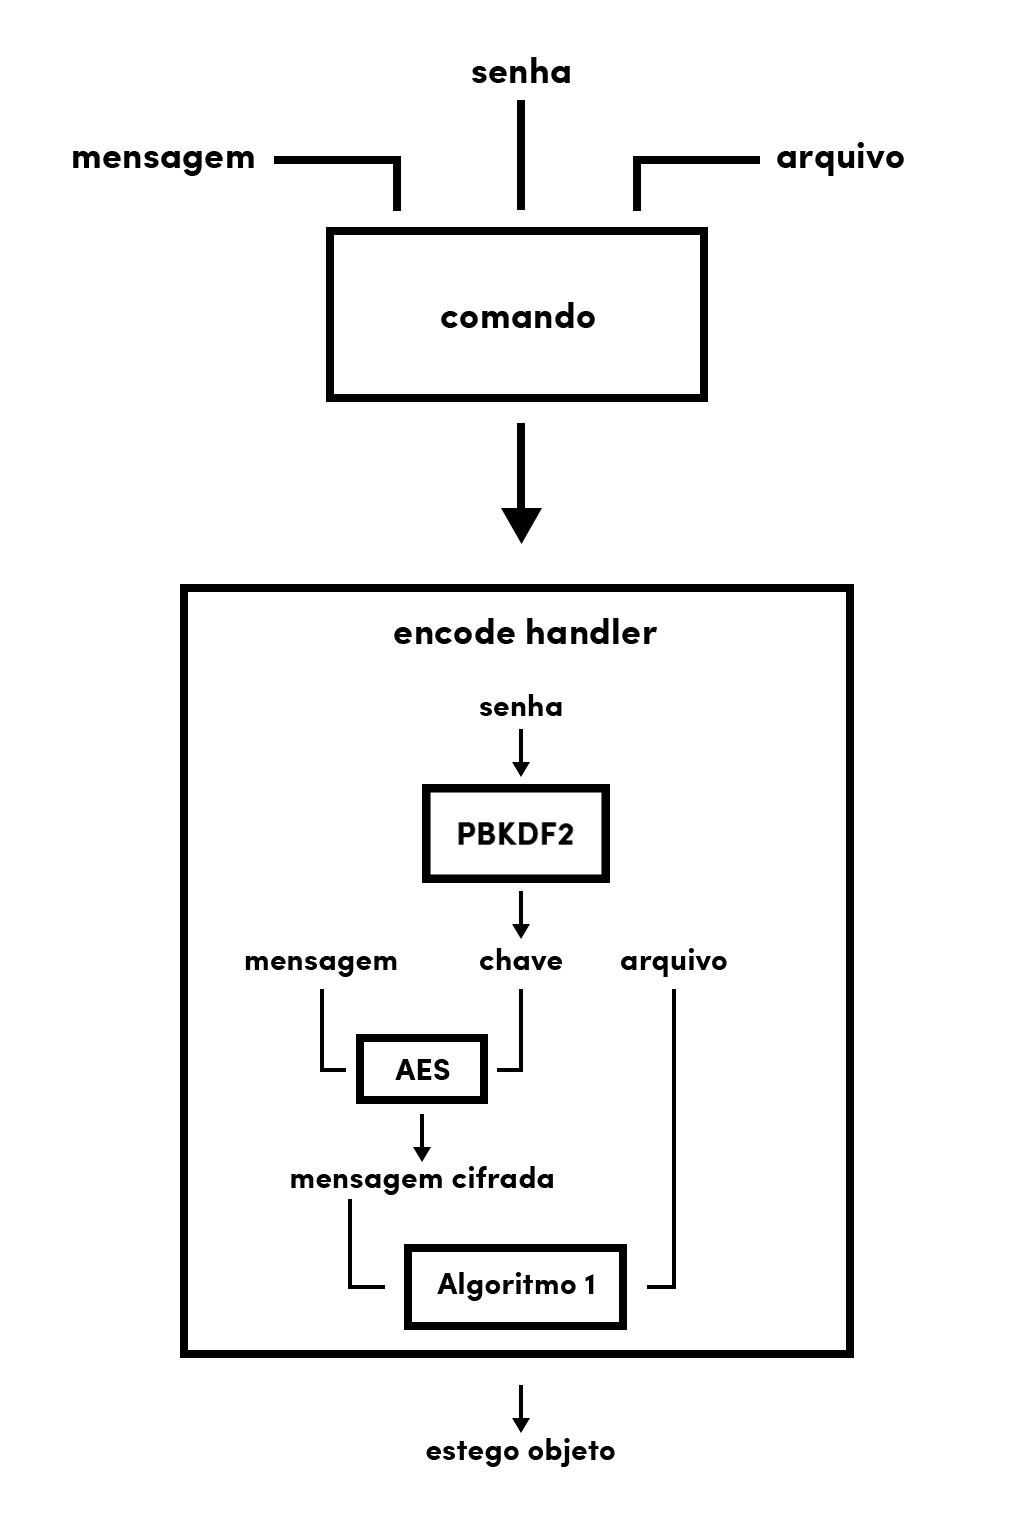
\includegraphics[width=10cm]{images/TCC4.png}
     \legend{Autor: Imagem produzida pelo Autor}
     \label{fig:encode}
\end{figure}

\subsubsection{\texttt{decode}}

O processo de decodificação é realizado de forma inversa a codificação, recebendo um arquivo binário que se presume ser um estego objeto criado com a mesma técnica e uma senha para descriptografar a mensagem. Inicialmente buscamos toda a mensagem criptografada contida no arquivo, utilizando o Algoritmo \ref{alg:two} como base até encontrar um caractere de parada, caso nenhum caractere de parada seja encontrado a aplicação levanta uma exceção alertando o usuário de que o arquivo não contém dados relevantes inseridos em si. Ao encontrar uma mensagem geramos uma chave a partir da senha utilizando PBKDF2 e o \textit{salt} contido no início da mensagem, ao ponto em que podemos descriptografar a mensagem utilizando o AES com a chave derivada e retornar a mensagem em texto plano para o usuário. O funcionamento completo do comando de codificação está ilustrado na Figura \ref{fig:decode}.

\begin{figure}[!tb]
     \centering
     \caption{Esquemático do funcionamento do processo de decodificação.}
     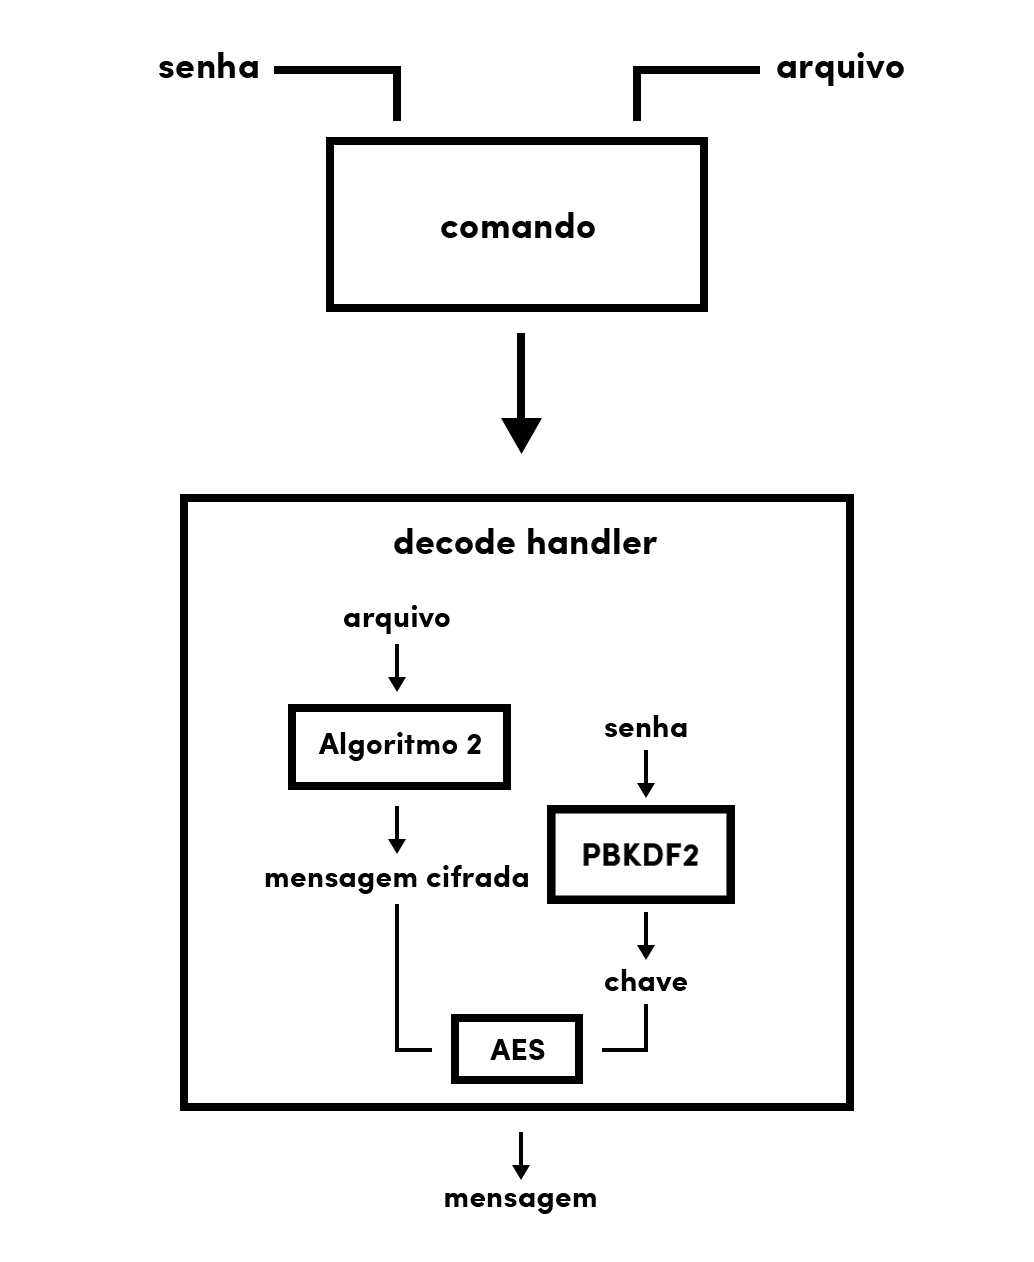
\includegraphics[width=10cm]{images/TCC5.png}
     \legend{Autor: Imagem produzida pelo Autor}
     \label{fig:decode}
\end{figure}

\subsection{Execução e Utilização da Aplicação}

Todo o código desenvolvido está disponível de forma pública no repositório \textit{git} localizado em \href{https://github.com/leviosar/tcc}{https://github.com/leviosar/tcc}, para instalar e executar é necessário possuir uma instalação da linguagem \textit{Python} em sua versão 3.11 ou superior e o gerenciador de pacotes \textit{Poetry}. Após clonar o repositório basta seguir as instruções contidas no arquivo \texttt{README.md} localizado no diretório \textit{src} do projeto.

Como mencionado anteriormente a aplicação implementada utiliza uma interface de linha de comando para responder à entrada do usuário, seguindo os padrões estabelecidos pela especificação POSIX para interpretação de opções, argumentos e caminhos de sistema, no trecho de código abaixo está descrita a utilização do programa a partir de sua interface 

\vspace{10mm}

\begin{lstlisting}[language=bash]
> python -m steganossaurus --help

Usage: python -m steganossaurus [OPTIONS] COMMAND [ARGS]...

Options:
  --help  Show this message and exit.

Commands:
  decode   Recover a message from the given FILE, decrypting it with a required password.
  encode   Embeds a message into the given FILE, encrypting it with a required password.
\end{lstlisting}

\vspace{10mm}

Primeiramente pode ser utilizado o argumento \texttt{\-\-help} sem nenhum comando para retornar mais informações sobre o programa, resultando em um curto guia de uso dos argumentos e disponibilização da lista de comandos.

\vspace{10mm}

\begin{lstlisting}[language=bash]
> python -m steganossaurus encode --help

Usage: python -m steganossaurus encode [OPTIONS] FILE MESSAGE

  Embeds a message into the given FILE, encrypting it with a required password.

Options:
  -o, --output PATH          Path to output file, created if not exists.
  --log-level                Level of data to de logged.
  --password                 Password used to encrypt the message.
  --help                     Show this message and exit.

> python -m steganossaurus encode ./input "steganographia" -o ./output

Password: **********
Repeat for confirmation: **********
Message was encoded at ./output
\end{lstlisting}

\vspace{10mm}

Em seguida o usuário pode chamar do comando \texttt{encode} com o argumento \texttt{\-\-help} que retorna instruções específicas para utilização do comando, como as opções disponíveis, a ordem e o nome dos argumentos. O comando \texttt{encode} então é invocado utilizando como argumentos um arquivo de entrada, uma mensagem para ser codificada pelo algoritmo e como opção um arquivo de saída. A aplicação então requer a digitação e confirmação de uma senha para o a mensagem criptografada e processa a solicitação do usuário, inserindo a mensagem no arquivo utilizando o Algoritmo \ref{alg:one} e gerando um estego-objeto no caminho fornecido.

\vspace{10mm}

\begin{lstlisting}[language=bash]
> python -m steganossaurus decode --help

Usage: python -m steganossaurus decode [OPTIONS] FILE

  Recover a message from the given FILE, decrypting it with a required password.

Options:
  --log-level               Level of data to de logged.
  --password TEXT           Password used to encrypt the message.
  --help                    Show this message and exit.

> python -m steganossaurus decode .\output

Password: **********
Repeat for confirmation: **********
Message found: steganographia
\end{lstlisting}

\vspace{10mm}

Para o processo de decodificação também é oferecida a opção de consultar a documentação do comando a partir da opção \texttt{\-\-help} que retorna todas as informações necessárias para a utilização do comando \texttt{decode}. Para finalizar o ciclo de vida da aplicação o usuário invoca o comando de decodificação passando como argumento o estego-objeto gerado no passo anterior, a aplicação solicita a senha e caso confirmada extrai a mensagem utilizando o Algoritmo \ref{alg:two}, descriptografa com a chave gerada a partir da senha informada e retorna a mensagem em texto plano para o usuário.



% ---


% ---
% 5 - Resultados
% ---
%\phantompart
\chapter{Discussão de Resultados}

Retornando ao problema dos prisioneiros apresentado no Capítulo 2 após termos apresentado tanto a técnica quanto sua implementação nos capítulos anteriores é possível realizar uma avaliação qualitativa dos resultados obtidos. Primeiramente podemos identificar que a implementação corresponde as prerrogativas do enunciado do problema, considerando que em uma comunicação a partir da metodologia proposta é utilizada uma chave privada definida previamente entre as duas partes, um objeto de cobertura arbitrário e se gera um estego objeto que pode ser trafegado em canal público. Devido à propriedade pseudoaleatória tanto dos bits gerados pela mensagem quanto operandos naturalmente codificados por instruções compiladas, é seguro afirmar que o carcereiro não teria a capacidade de identificar um subtexto malicioso dentro do estego objeto, e como assumimos a priori que a vigilância seria passiva, a destruição da integridade da mensagem não é preocupação deste estudo.

Existem ainda ataques comuns a classe de técnica utilizada na implementação deste trabalho descritos na litetura, que buscam encontrar assinaturas ou características comuns à transformações de código aplicadas \cite{ICISC04}. Um atacante buscando detectar essas assinaturas pode buscar pela presença de instruções pouco utilizadas em uma arquitetura a fim de identificar um padrão de substituição. Entretanto como o Algoritmo \ref{alg:one} não substitui instruções, trabalhando apenas com substituição de operandos, não há risco de ter essa propriedade explorada. Outra possibilidade é a detecção de uma frequência anormal de um certo tipo de instruções, também descartada pelo motivo anterior. Por fim, o atacante pode inspecionar o comportamento dos \textit{jumps} entre endereços do programa, buscando valores discrepantes que não seria naturalmente endereçados por compiladores. Tal vulnerabilidade também é inefetiva contra a aplicação desenvolvida pela ausência da alteração de valores imediatos em instruções de controle.

Nota-se então que os ataques já observados na bibliografia disponível não tem a capacidade de detectar as transformações realizadas pelo algoritmo proposto, o que não significa dizer que o mesmo seja indetectável, considerando que os ataques foram planejados para expor vulnerabilidades em técnicas aplicadas na arquitetura \textit{x86} que possui uma gama de possibilidades de alteração superior. Em fato, a eficiência de codificação de instruções da arquitetura RISC-V simultâneamente favorece a avaliação qualitativa de transformações binárias enquanto desfavorece uma avaliação quantitativa, reduzindo o número de permutações equivalentes dentro do programa e tornando a codificação de informações mais silenciosa porém menos eficiente.
% ---

% ---
% 6 - Conclusão
% ---
%\phantompart
% ----------------------------------------------------------
\chapter{Conclusão}
% ----------------------------------------------------------

O campo da esteganografia evolui pela história humana antes mesmo do cunho de seu próprio termo, entretanto suas aplicações com utilização voltada para formatos de código compilado ainda não possuem técnicas tão difundidas em comparação com outras categorias de objetos de cobertura, tornando a própria execução deste trabalho um desafio considerável. Após revisar e analisar quase 30 anos de estudos formais na área foi possível utilizar os conhecimentos e técnicas obtidas para aplicar uma metodologia de codificação de dados já proposta em uma arquitetura ainda não explorada com sucesso.

O algoritmo proposto é capaz de explorar redundâncias provenientes de operações comutativas na arquitetura RISC-V para codificar um bit a cada operação suportada e sua implementação foi desenvolvida de forma a minimizar o uso de recursos para possibilitar a execução eficiente mesmo em arquivos de grande porte. Apesar do resultado positivo na viabilidade da aplicação é necessário ressaltar que sua eficácia é reduzida em comparação com arquiteturas CISC devido a sua própria filosofia de elaboração, fornecendo um espaço útil de codificação com ao menos um nível de grandeza inferior. 

Ao avaliar a técnica por outro prisma, relevando a baixa taxa de codificação e focando primariamente na detectabilidade e corretude quanto ao problema dos prisioneiros, entende-se que os pontos negativos podem ser mitigados com o uso do algoritmo em situações específicas, aproveitando-se da dificuldade em revelar a mensagem sem conhecimento da chave para inserir mensagens de tamanho reduzido em arquivos. Tais situações podem ser exploradas para embutir assinaturas e identificadores em \textit{softwares} distribuídos comercialmente com o objetivo de rastrear violações de direitos autorais no combate à pirataria.

\section{Trabalhos Futuros}

A execução deste trabalho revela algumas portas em aberto para a evolução das técnicas de esteganografia em código compilado, principalmente considerando a arquitetura RISC-V. Durante a revisão bibliográfica foram encontrados pontos de exploração com potencial para codificação de dados, que poderiam ser unidos a técnica desenvolvida para incrementar a taxa de codificação. Inicialmente existe a possibilidade de explorar as instruções \texttt{HINT}, reservadas no espaço de endereçamento da arquitetura como livres para uso de implementações, normalmente utilizadas para otimizações de performance mas que poderiam ser subvertidas para carregar bits de mensagens. Além disso, no decorrer da pesquisa realizada o foco foi aplicar transformações diretamente no conjunto de instruções base da arquitetura, deixando de fora diversas extensões de propósitos específicos que apesar de possuírem frequência menor de aparecimento em um programa arbirtrário podem aumentar a taxa total de codificação de dados.

Ainda no escopo da arquitetura RISC-V e da implementação atual, levando em consideração que a validação de detectabilidade da técnica foi realizada a partir de ataques comuns direcionados a binários compilados para \textit{x86}, é necessário expo-la a técnica à uma gama maior de ataques que possam expor vulnerabilidades específicas da arquitetura para reforçar a confiabilidade do algoritmo.

Por fim, existem outras arquiteturas RISC amplamente utilizadas em dispositivos ao redor do mundo, principalmente da família ARM nas quais os conhecimentos adquiridos podem ser aplicados, resultando na portabilidade da técnica para um leque maior de usuários e possivelmente em resultados superiores se considerarmos que o endereçamento do RISC-V possui uma maior rigidez aos princípios RISC.
% ---

% ----------------------------------------------------------
% ELEMENTOS PÓS-TEXTUAIS
% ----------------------------------------------------------
\postextual
% ----------------------------------------------------------

% ----------------------------------------------------------
% Referências bibliográficas
% ----------------------------------------------------------
\begingroup
    \SingleSpacing\printbibliography[title=REFERÊNCIAS]
\endgroup

% ----------------------------------------------------------
% Glossário
% ----------------------------------------------------------
%
% Consulte o manual da classe abntex2 para orientações sobre o glossário.
%
%\glossary

% ----------------------------------------------------------
% Apêndices
% ----------------------------------------------------------

% ---
% Inicia os apêndices
% ---
\begin{apendicesenv}
%	\partapendices* 
	% % ----------------------------------------------------------
\chapter{Descrição}
% ----------------------------------------------------------

Textos elaborados pelo autor, a fim de completar a sua argumentação. Deve ser precedido da palavra APÊNDICE, identificada por letras maiúsculas consecutivas, travessão e pelo respectivo título. Utilizam-se letras maiúsculas dobradas quando esgotadas as letras do alfabeto. 

\begin{quadro}[htb]
	\centering
	\caption{\label{qua:Quadro_2}Modelo A.}	
\begin{tabular}{|l|l|}
\hline
xxxx              & yyyyyyyyyyyyyyy    \\
\hline
xxxx              & yyyyyyyyyyyyyyy    \\
\hline
xxxx              & yyyyyyyyyyyyyyy    \\
\hline
xxxx              & yyyyyyyyyyyyyyy    \\
\hline
xxxx              & yyyyyyyyyyyyyyy    \\
\hline
xxxx              & yyyyyyyyyyyyyyy    \\
\hline
xxxx              & yyyyyyyyyyyyyyy    \\
\hline
rrrrrrrrrrrrrrrrr & eeeeeeeeeeeeeeeee  \\
\hline
xxxx              & yyyyyyyyyyyyyyy    \\
\hline
xxxx              & yyyyyyyyyyyyyyy    \\
\hline
rrrrrrrrrrrrrrrrr & eeeeeeeeeeeeeeeee  \\
\hline
xxxx              & yyyyyyyyyyyyyyy    \\
\hline
                  & ttttttttttttttttt  \\
\hline
rrrrrrrrrrrrrrrrr & eeeeeeeeeeeeeeeee  \\
\hline
ttttttttttttt     &                    \\
\hline
rrrrrrrrrrrrrrrrr & eeeeeeeeeeeeeeeee  \\
\hline
rrrrrrrrrrrrrrrrr & eeeeeeeeeeeeeeeee  \\
\hline
                  & gggggggggggggggggg \\
\hline
rrrrrrrrrrrrrrrrr & eeeeeeeeeeeeeeeee  \\
\hline
rrrrrrrrrrrrrrrrr & eeeeeeeeeeeeeeeee  \\
\hline
rrrrrrrrrrrrrrrrr & eeeeeeeeeeeeeeeee  \\
\hline
rrrrrrrrrrrrrrrrr & eeeeeeeeeeeeeeeee  \\
\hline
\end{tabular}
\fonte{Elaborada pelo autor (2016).}
\end{quadro}
\end{apendicesenv}
% ---


% ----------------------------------------------------------
% Anexos
% ----------------------------------------------------------

% ---
% Inicia os anexos
% ---
\begin{anexosenv}
%	\partanexos*
	% % ----------------------------------------------------------
\chapter{Descrição}
% ----------------------------------------------------------

São documentos não elaborados pelo autor que servem como fundamentação (mapas, leis, estatutos). Deve ser precedido da palavra ANEXO, identificada por letras maiúsculas consecutivas, travessão e pelo respectivo título. Utilizam-se letras maiúsculas dobradas quando esgotadas as letras do alfabeto. 

\end{anexosenv}

%---------------------------------------------------------------------
% INDICE REMISSIVO
%---------------------------------------------------------------------
%\phantompart
%\printindex
%---------------------------------------------------------------------

\end{document}
